% Created 2024-07-08 Mon 18:42
% Intended LaTeX compiler: pdflatex
\documentclass[10pt,table,dvipsnames,compress]{beamer}
\usepackage[utf8]{inputenc}
\usepackage[T1]{fontenc}
\usepackage{graphicx}
\usepackage{longtable}
\usepackage{wrapfig}
\usepackage{rotating}
\usepackage[normalem]{ulem}
\usepackage{amsmath}
\usepackage{amssymb}
\usepackage{capt-of}
\usepackage{hyperref}
\usetheme{default}
\useinnertheme{rounded}
\useoutertheme[subsection=false]{miniframes}
\date{}
\title{Using the deforisk QGIS plugin for making and comparing deforestation risk maps}
\title[deforisk QGIS plugin]{Using the \texttt{deforisk} QGIS plugin for making and comparing deforestation risk maps}
\definecolor{darkgreen}{RGB}{34,139,34} % vert moyen
\usepackage{float}
\usepackage{lmodern}
\usepackage{pgf}
\usepackage{color}
\usepackage[english,french]{babel}
\definecolor{vertmoyen}{RGB}{51,110,23} % vert moyen
\definecolor{blueFRB}{HTML}{31859c}
\usecolortheme[named=blueFRB]{structure}
\usepackage{tabularx} % varier la largeur du tableau
\usepackage{layout}
\setlength{\LTleft}{-5cm plus 1 fill}
\setlength{\LTright}{-5cm plus 1 fill}
\usepackage{booktabs}
\usepackage{arydshln} %% dashlines for tabular
\newcommand{\logit}{\text{logit}}
\newcommand{\bs}[1]{\boldsymbol{#1}}
\newcommand{\R}{\textnormal{\sffamily\bfseries R}}
\newcommand{\pkg}[1]{{\fontseries{b}\selectfont #1}}
\newcolumntype{C}[1]{>{\centering\arraybackslash}m{#1}}

\setbeamertemplate{footline}[frame number]
\setbeamertemplate{frametitle}{%
\usebeamerfont{frametitle}\insertframetitle%
\vphantom{g} % To avoid fluctuations per frame
\par
\centering 
\includegraphics[width=\textwidth]{figs/Barre_couleur}
}
\beamertemplatenavigationsymbolsempty

% Logo
\newif\ifplacelogo % create a new conditional
\logo{\ifplacelogo
\includegraphics[width=0.5\textwidth]{figs/partners_logos}\fi}

%Call table of contents at the beginning of each section
\AtBeginSection[]{
\placelogotrue
\begin{frame}
\frametitle{Outline}
\begin{columns}[c]
\begin{column}{0.5\textwidth}
\tableofcontents[sections=1,currentsection]
\vspace{0.5cm}
\tableofcontents[sections=2,currentsection]
\vspace{0.5cm}
\tableofcontents[sections=3,currentsection]
\end{column}
\begin{column}{0.5\textwidth}
\tableofcontents[sections=4,currentsection]
\vspace{0.5cm}
\tableofcontents[sections=5,currentsection]
\end{column}
\end{columns}
\end{frame}
\placelogofalse
}

\AtBeginSubsection[]{}

\hypersetup{
colorlinks=true,
linkcolor=Black,
filecolor=Maroon,
citecolor=Blue,
urlcolor=Maroon}

% Disable monospaced font for URLs
\urlstyle{same}

\hypersetup{
 pdfauthor={Ghislain Vieilledent},
 pdftitle={Using the deforisk QGIS plugin for making and comparing deforestation risk maps},
 pdfkeywords={},
 pdfsubject={},
 pdfcreator={Emacs 29.3 (Org mode 9.6.15)}, 
 pdflang={English}}
\begin{document}

% po4a: environment frame
% po4a: environment column
% po4a: environment columns
% po4a: environment block {_}
% po4a: command -textcolor {}{_}
% po4a: command textbf {_}

% {
%   % Use background image
%   \usebackgroundtemplate{%
%     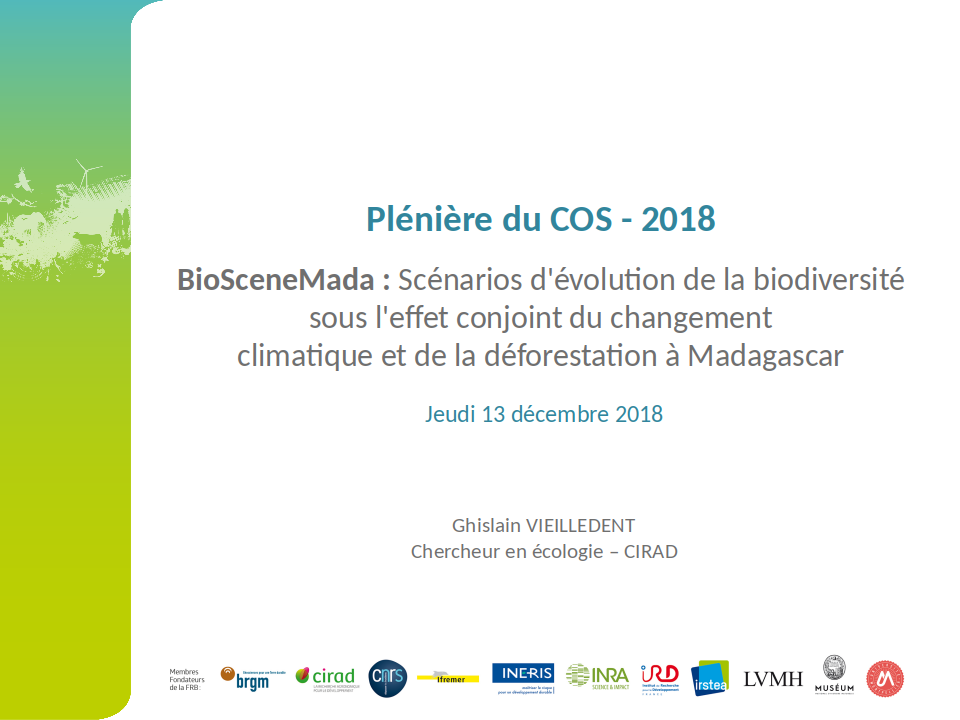
\includegraphics[height=\paperheight,width=\paperwidth]{figs/Masque.png}
%   }
%   \setbeamertemplate{navigation symbols}{}
%   % Remove shadow from block
%   \setbeamertemplate{blocks}[rounded][shadow=false]
%   \begin{frame}[plain]
%   \end{frame}
% }

% Title page
{
  \setbeamertemplate{navigation symbols}{}
  \begin{frame}[plain, noframenumbering]
  \begin{center}
  \small{\textbf{FAO workshop -- Santa Marta (Colombia), July 2024}}
  \end{center}
  \vspace{-0.5cm}
  \titlepage % Presentation first page
  \vspace{-3cm}
  \begin{center}
    
\includegraphics[width=\textwidth]{figs/Barre_couleur}
    
    \vspace{0.25cm}
    
    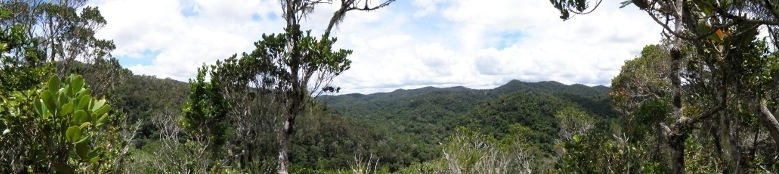
\includegraphics[width=10cm]{figs/Banniere}
    
    \small{Ghislain VIEILLEDENT$^{1}$\hspace{0.25cm}Thomas ARSOUZE$^{1}$\hspace{0.25cm}FAO team$^{2}$}
      
    \vspace{0.25cm}
    
    {\scriptsize
      \begin{tabular}{l}
        $[1]$ \textbf{Cirad} UMR AMAP, $[2]$ \textbf{FAO} Rome and Latin America
      \end{tabular}
    }
    
    
\includegraphics[width=0.8\textwidth]{figs/partners_logos}
    
  \end{center}
  \end{frame}
}

% %%%%%%%%%%%%%%%%%%%%%%%%%%%%%%%%%%%%%%%%%%%%%%%%%%%%%%%%%%%%%%%%

\placelogotrue
\begin{frame}
  \frametitle{Outline}
  \begin{columns}[c]
    \begin{column}{0.5\textwidth}
      \tableofcontents[sections=1]
      \vspace{0.5cm}
      \tableofcontents[sections=2]
      \vspace{0.5cm}
      \tableofcontents[sections=3]
    \end{column}
    \begin{column}{0.5\textwidth}
        \tableofcontents[sections=4]
        \vspace{0.5cm}
        \tableofcontents[sections=5]
    \end{column}
  \end{columns}
\end{frame}
\placelogofalse

\section{The deforisk QGIS plugin}
\label{sec:orga583b1a}

\subsection{Aim and specificities}
\label{sec:orgc8a08d6}

\begin{frame}[label={sec:org46f9bdf}]{Aims}
\end{frame}

\begin{frame}[label={sec:org9745e5e}]{Specificities}
\end{frame}

\begin{frame}[label={sec:org08148c9},fragile]{Python based}
 \textbf{Python based.} The \texttt{deforisk} plugin relies on four Python packages developed specifically for modelling deforestation: \texttt{geefcc}, \texttt{pywdpa}, \texttt{forestatrisk}, and \texttt{riskmapjnr}.

\begin{itemize}
\item \texttt{geefcc}: make forest cover change maps from Google Earth Engine (GEE).
\item \texttt{pywdpa}: downloading protected areas from the World Database on Protected Areas (WDPA).
\item \texttt{forestatrisk}: model deforestation and predict the spatial deforestation.
\item \texttt{riskmapjnr}: risk maps following Verra JNR methodologies.
\end{itemize}

\begin{center}
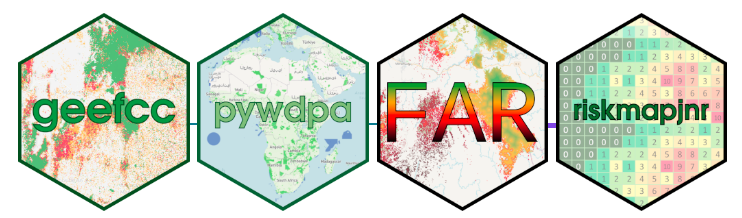
\includegraphics[width=0.7\textwidth]{figs/logos-packages.png}
\end{center}
\end{frame}

\begin{frame}[label={sec:org084c211},fragile]{Processing raster by blocks}
 \begin{itemize}
\item \textbf{Processing raster by blocks.} Raster files of forest cover change and explanatory variables might occupy a space of several gigabytes on disk. Processing such large rasters in memory can be prohibitively intensive on computers with limited RAM. Functions used in the \texttt{deforisk} plugin process large rasters by blocks of pixels representing subsets of the raster data. This makes computation efficient, with low memory usage. Reading and writing subsets of raster data is done by using functions from GDAL, a dependency of the plugin. Numerical computations on arrays are performed with the NumPy Python package, whose core is mostly made of optimized and compiled C code that runs quickly.
\end{itemize}
\end{frame}

\begin{frame}[label={sec:orgb49bad9},fragile]{Running tasks in parallel}
 \begin{itemize}
\item \textbf{Running tasks in parallel.} State-of-the-art approach to select the best deforestation risk map and forecast deforestation implies comparing various models, fit the models using forest cover change over different time periods and predict the deforestation risk at several dates. This implies repeating a high number of tasks. To save computation time, the \texttt{deforisk} plugin use the QGIS task manager which allows running several analysis in parallel.
\end{itemize}
\end{frame}

\subsection{Website and documentation}
\label{sec:org72981d7}

\begin{frame}[label={sec:org91a1837}]{Website and documentation}
\end{frame}

\subsection{Installation}
\label{sec:org2ce624d}

\begin{frame}[label={sec:org695b58f}]{Installation}
\end{frame}

\section{Data preparation}
\label{sec:orgd689b08}

\subsection{Forest cover change data}
\label{sec:org0f3c058}

\begin{frame}[label={sec:orgb5717aa}]{GFC dataset}
\end{frame}

\begin{frame}[label={sec:org5354625}]{TMF dataset}
\begin{itemize}
\item Full Landsat archive (1982--2022), 30m pixel, time-series analysis.
\item Classification tree based on expert knowledge.
\item Tropical deforestation was underestimated (-33\% in 2000--2012, Hansen
et al. 2013).
\item Maps and data: \url{https://forobs.jrc.ec.europa.eu/TMF/}.
\end{itemize}

\vspace{0.25cm}

\begin{center}
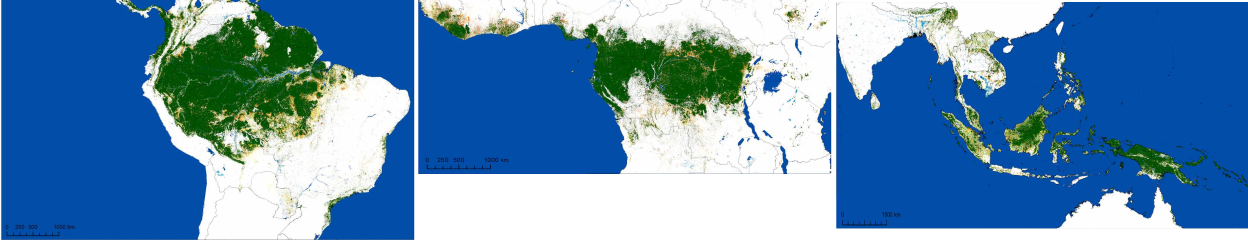
\includegraphics[width=\textwidth]{figs/Vancutsem2021-maps-wide.png}
\end{center}
\end{frame}

\begin{frame}[label={sec:org9cc5c5f}]{TMF dataset}
\begin{itemize}
\item Precise enough to visually identify the causes of deforestation
(logging, fires, agriculture)
\end{itemize}

\begin{center}
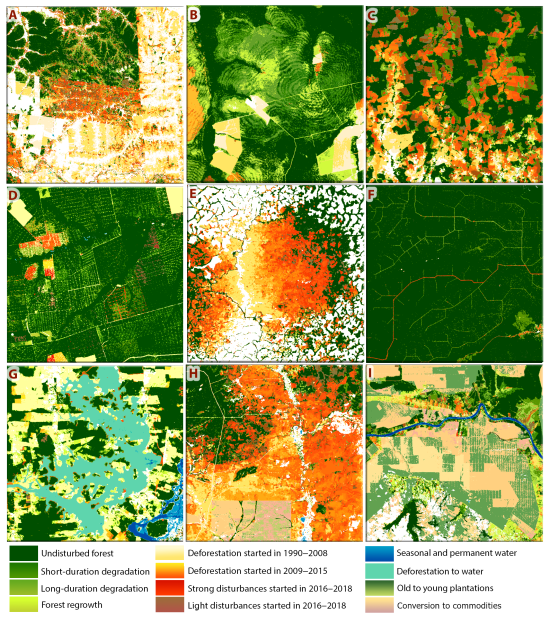
\includegraphics[width=0.5\textwidth]{figs/Vancutsem2021-patterns.png}
\end{center}
\end{frame}

\subsection{Spatial explanatory variables}
\label{sec:org227c2a6}

\begin{frame}[label={sec:org453b1f7}]{Spatial variables}
\begin{itemize}
\item Height explanatory variables
\end{itemize}

\begin{center}
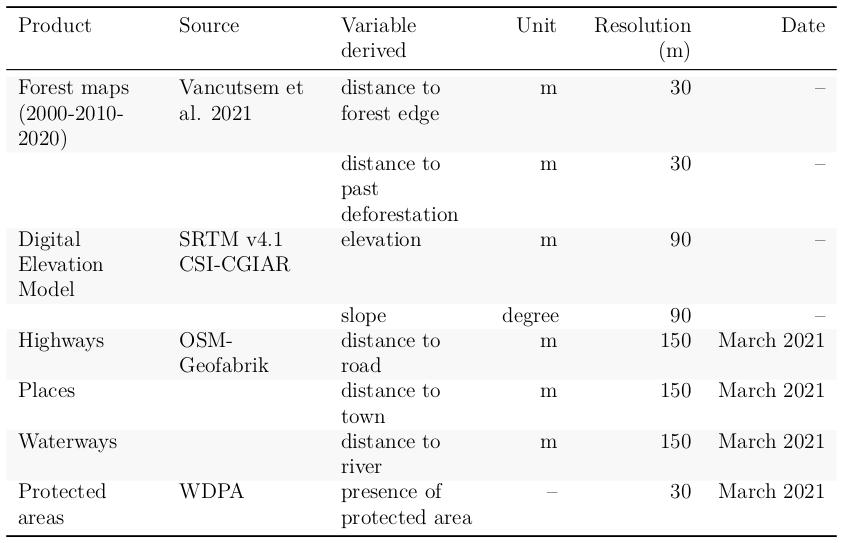
\includegraphics[width=0.75\textwidth]{figs/variables-tab.png}
\end{center}
\end{frame}

\begin{frame}[label={sec:org40757fa}]{Spatial variables}
\begin{center}
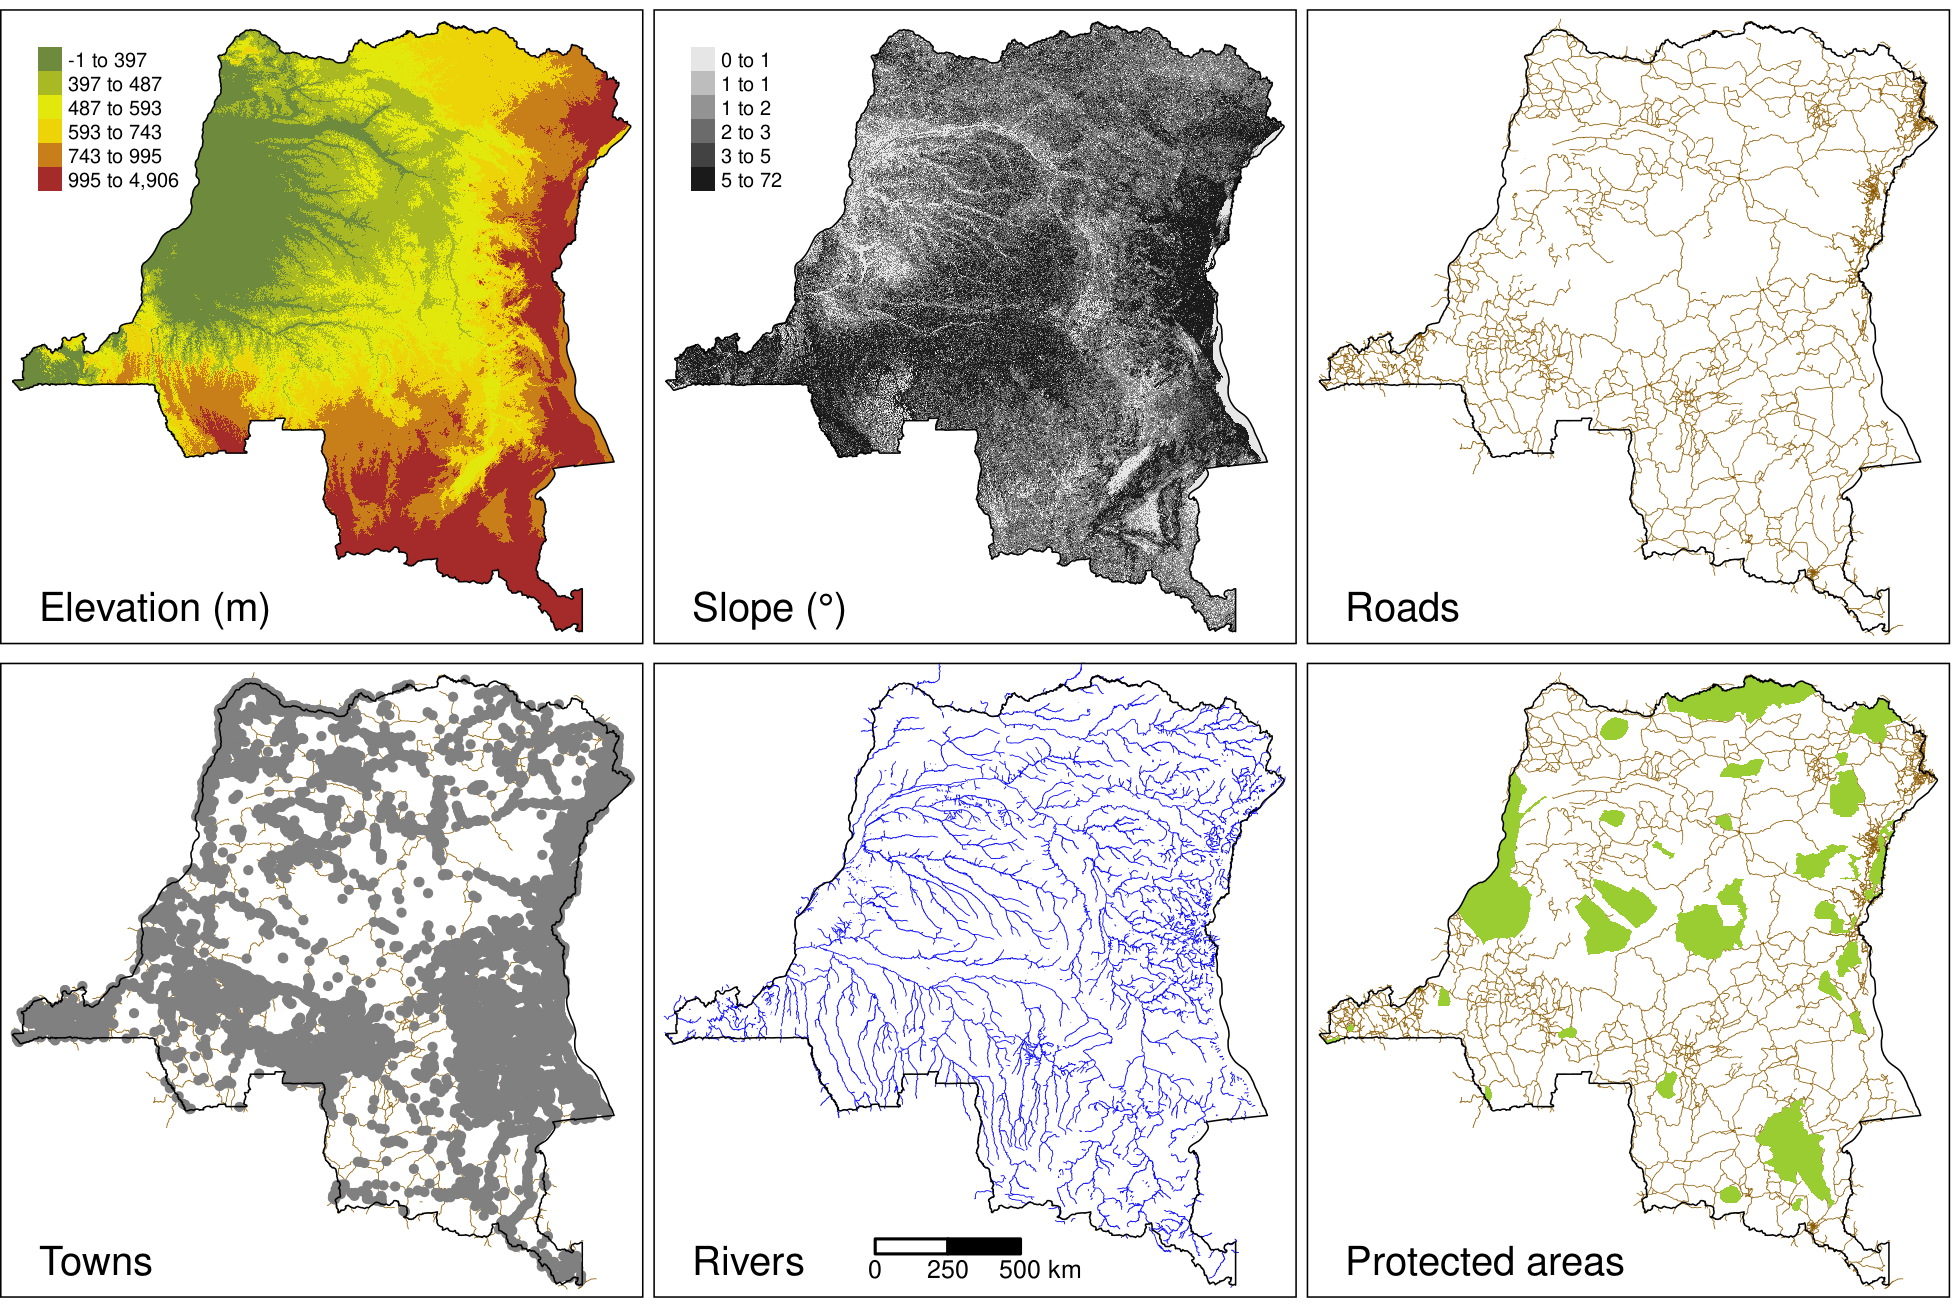
\includegraphics[width=0.8\textwidth]{figs/sm/var.png}
\end{center}

\centering \textbf{Spatial explanatory variables in DRC}
\end{frame}

\begin{frame}[label={sec:orge28d3b6}]{Roads}
\begin{itemize}
\item OpenStreetMap (OSM)
\item ``motorway'', ``trunk'', ``primary'', ``secondary'' and ``tertiary'' roads
\item 3.6 million roads from OSM
\end{itemize}

\begin{center}
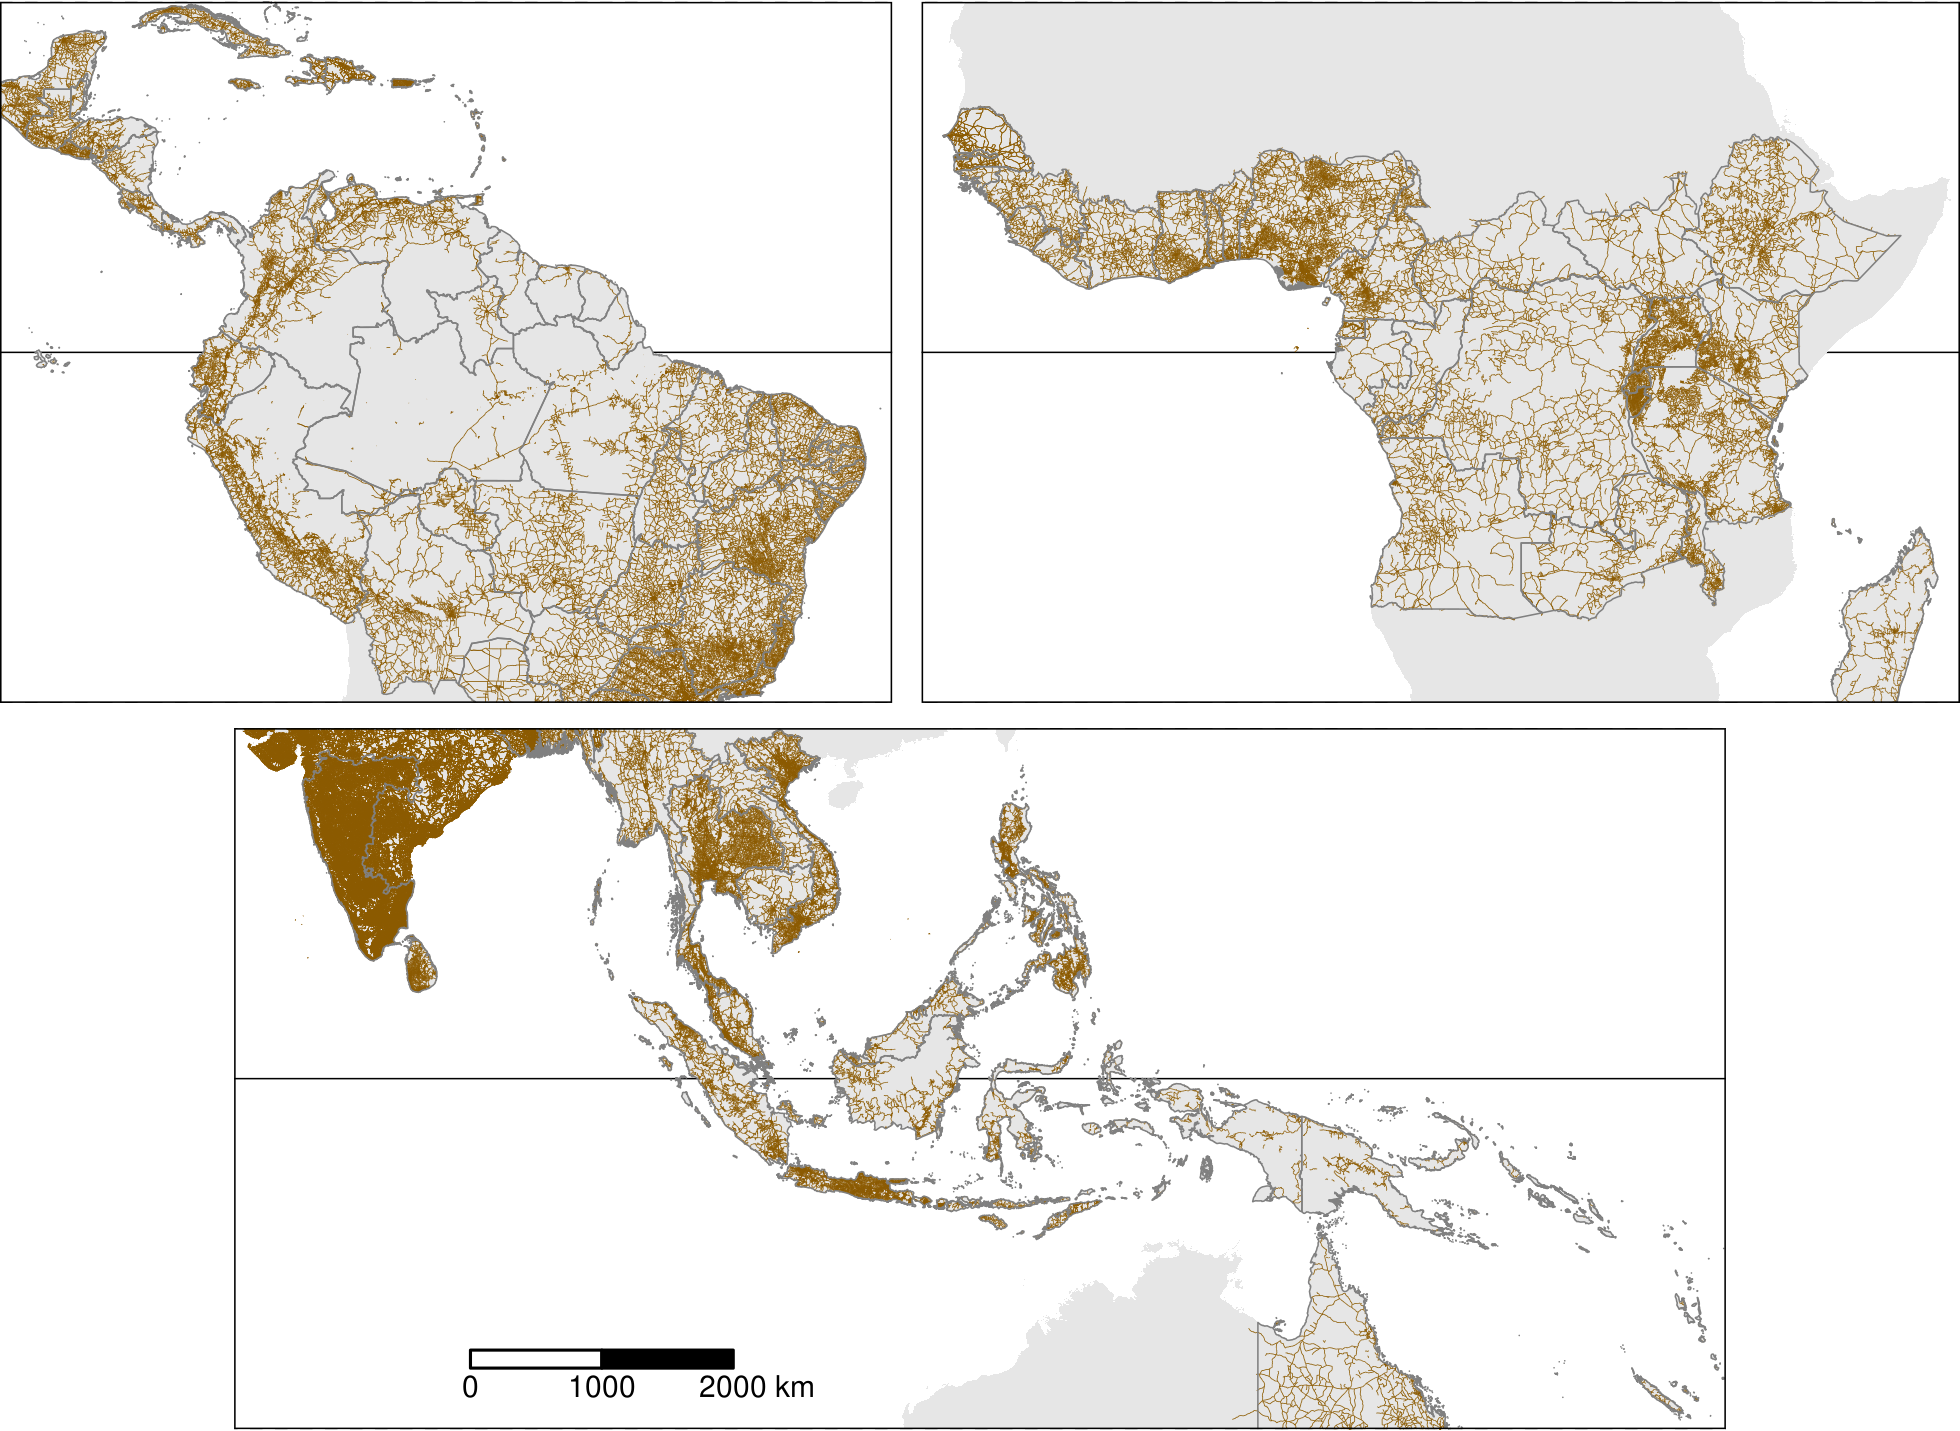
\includegraphics[width=0.7\textwidth]{figs/sm/roads.png}
\end{center}
\end{frame}

\begin{frame}[label={sec:org9ce4fc8}]{Protected areas}
\begin{itemize}
\item PA status: ``Designated'', ``Inscribed'', ``Established'', or ``Proposed''
before 1\textsuperscript{st} January 2010
\item 85,000 protected areas from WDPA
\end{itemize}

\begin{center}
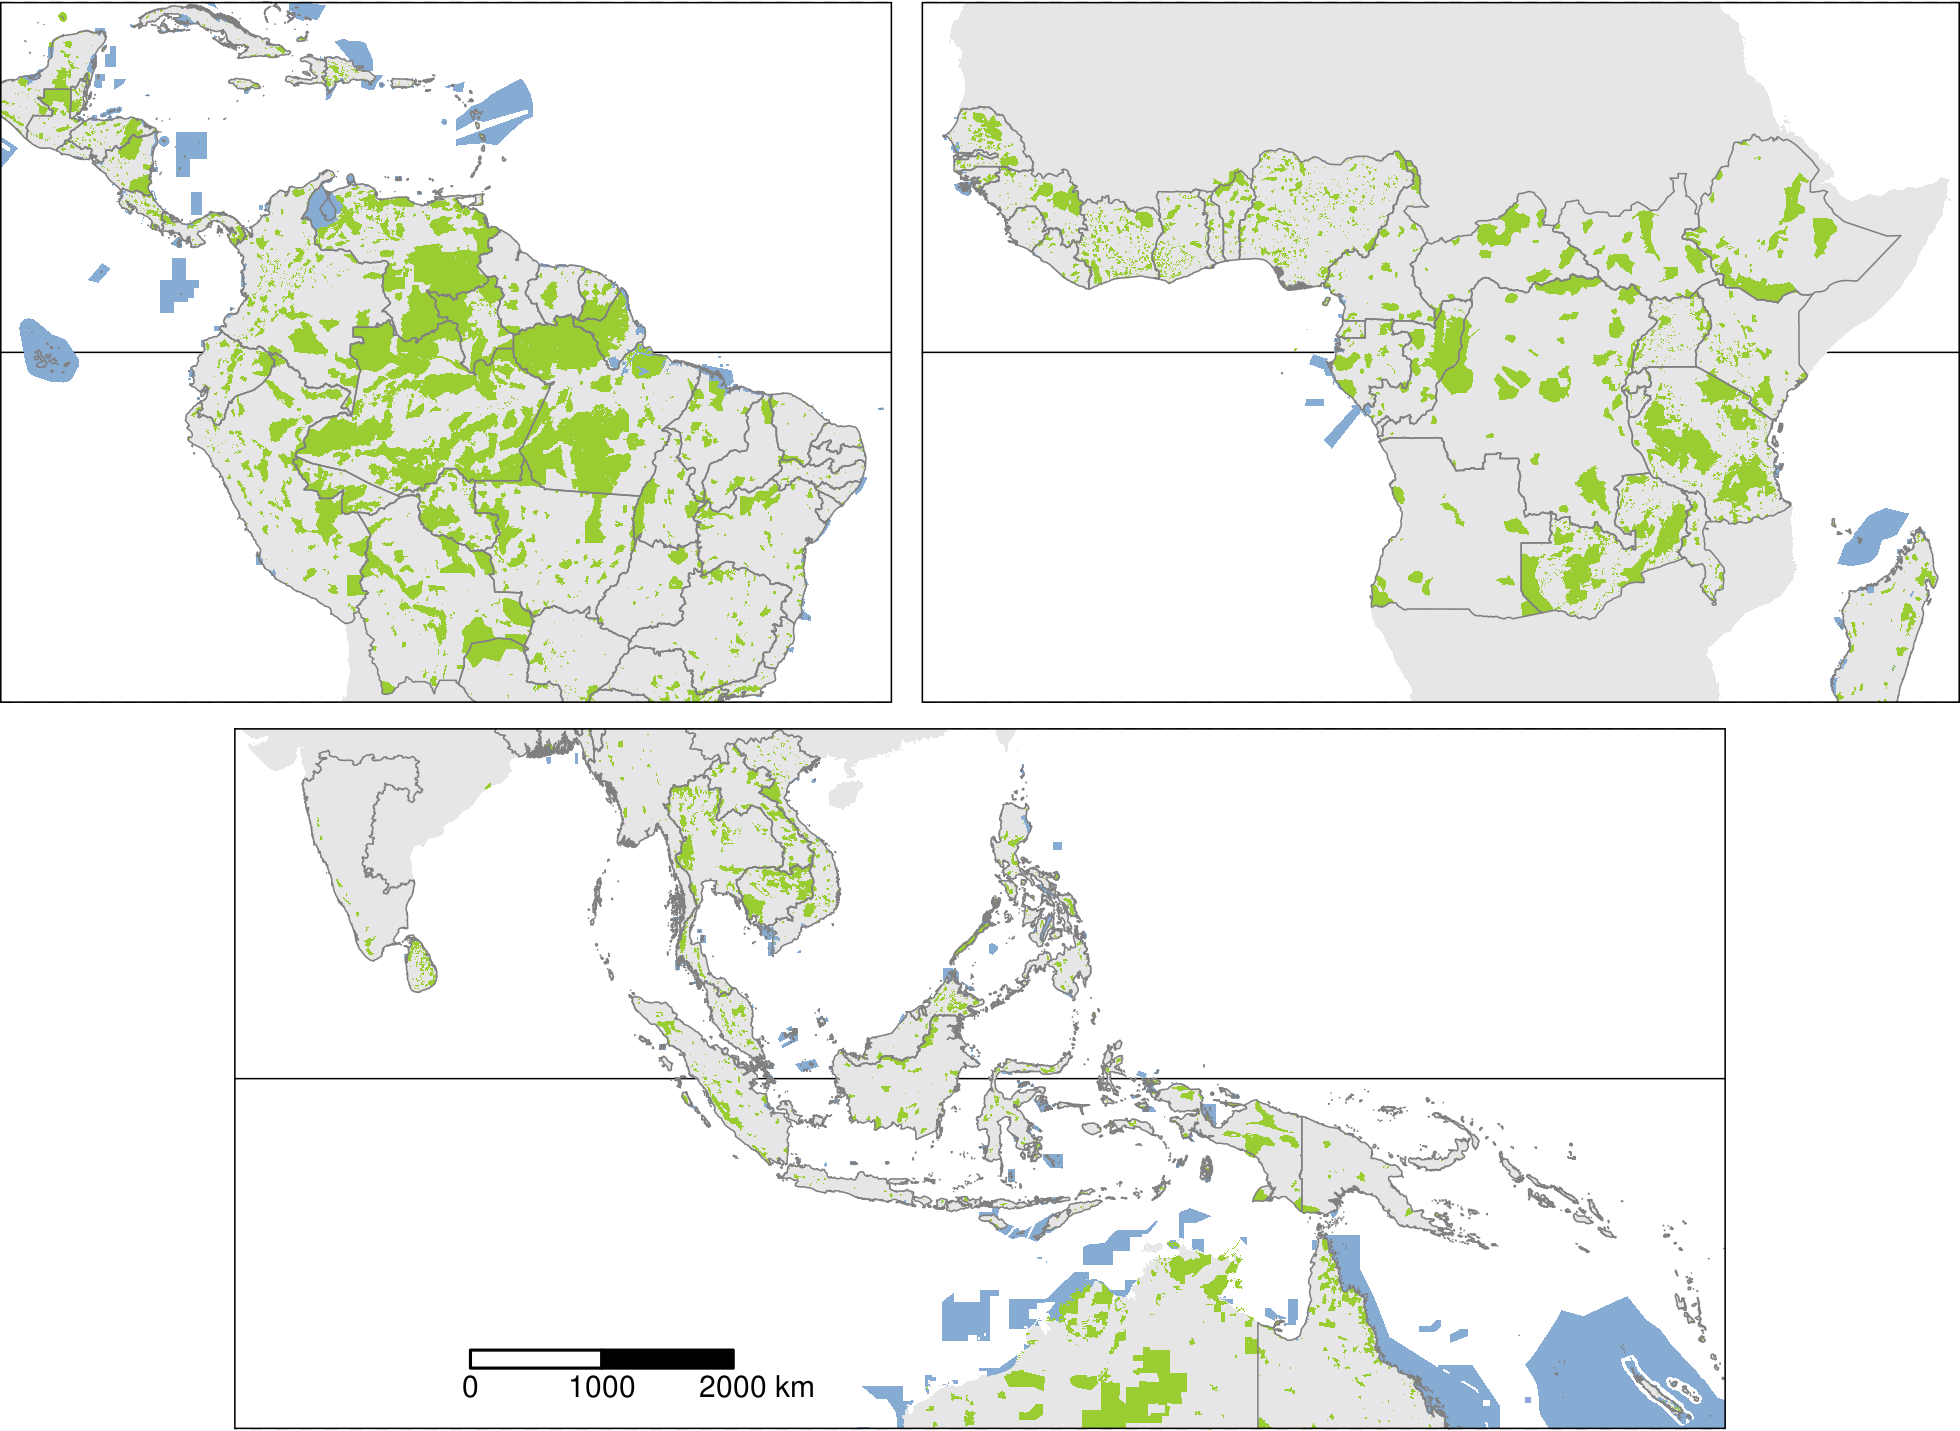
\includegraphics[width=0.7\textwidth]{figs/sm/pa.png}
\end{center}
\end{frame}

\subsection{Sampling}
\label{sec:org28b713c}

\begin{frame}[label={sec:orgb2dd237}]{Sampling}
\begin{itemize}
\item Stratified sampling between deforested/non-deforested pixels in
2010--2020
\item Total number of points proportional to the forest cover in 2010 (from
20,000 to 100,000 points per study area)
\end{itemize}

\begin{center}
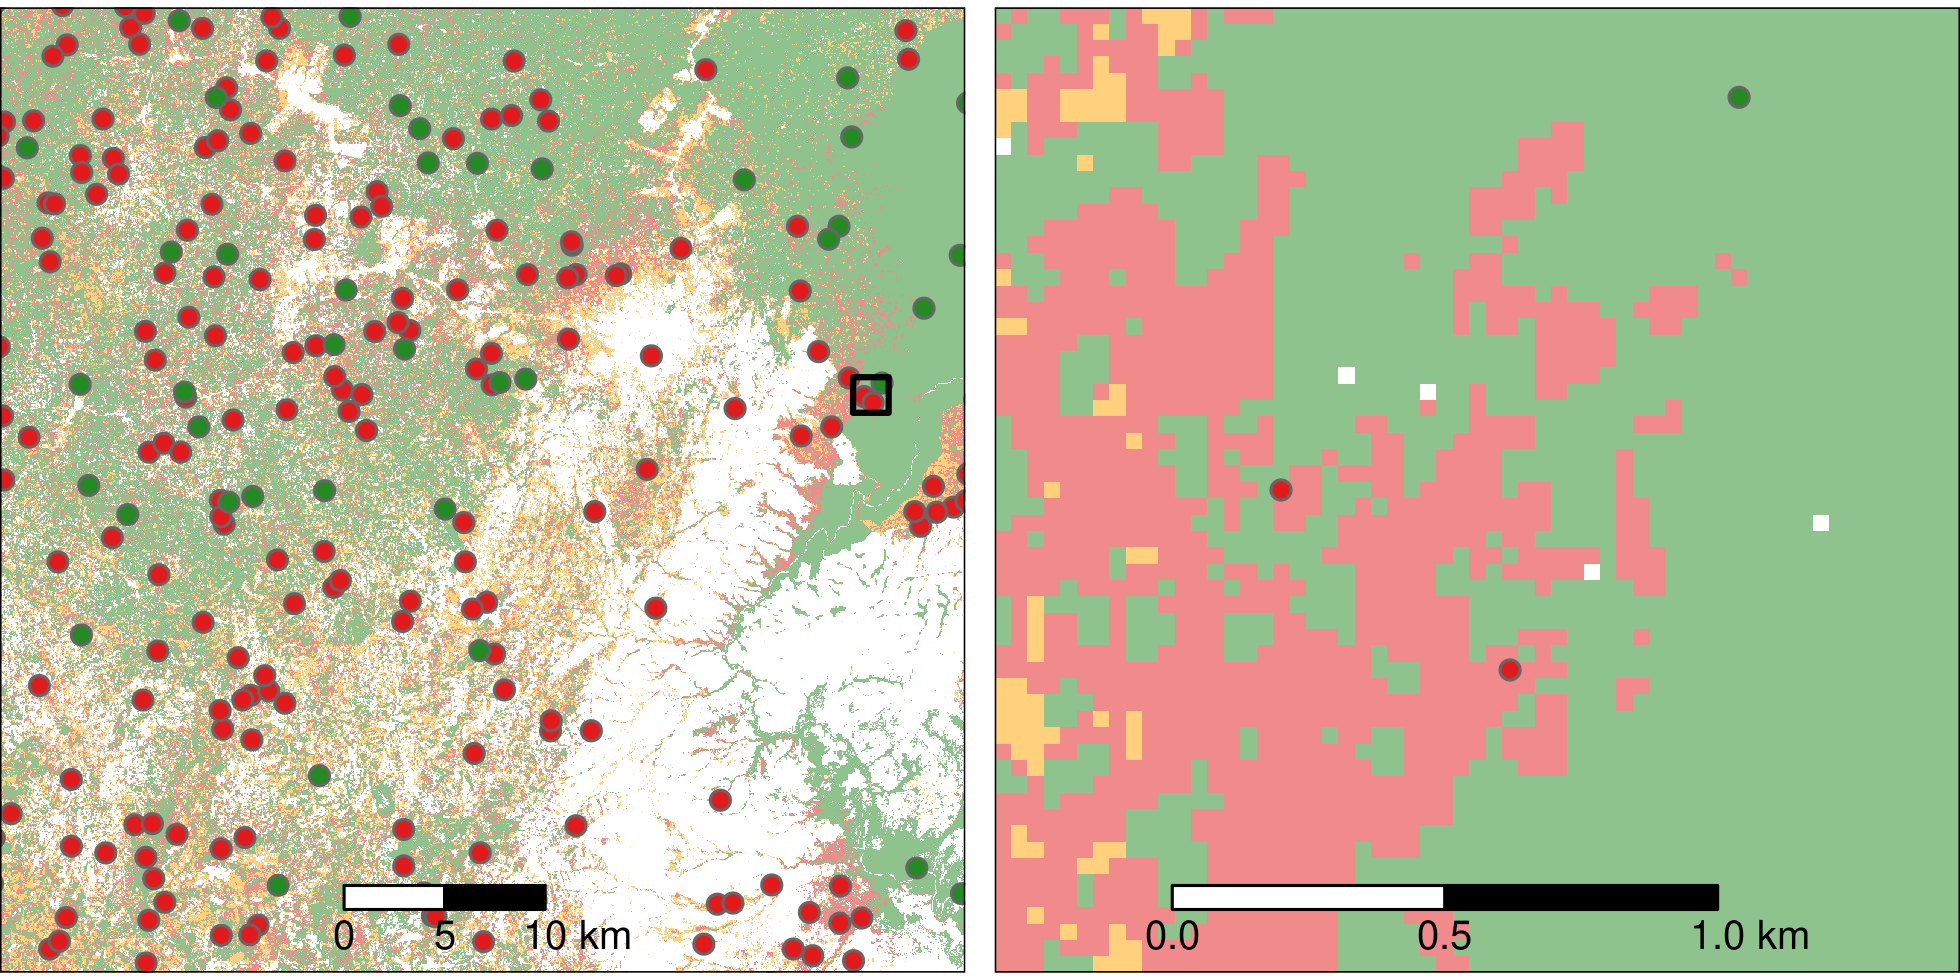
\includegraphics[width=0.7\textwidth]{figs/sm/sample.png}
\end{center}
\end{frame}

\section{Models and validation}
\label{sec:org35f1d54}

\subsection{Benchmark model}
\label{sec:org24b7bb0}

\begin{frame}[label={sec:orgaf18810}]{Benchmark model}
\end{frame}

\subsection{Forestatrisk models}
\label{sec:org21a965e}

\begin{frame}[label={sec:orgfd062d7}]{Forestatrisk models}
\end{frame}


\begin{frame}[label={sec:orgd4bc244}]{iCAR model}
\begin{columns}
\begin{column}{0.5\columnwidth}
A logistic regression model with iCAR process

\begin{equation*}
\begin{split}
  y_i \sim \mathcal{B}ernoulli(\theta_i)\\
  \text{logit}(\theta_i) = \alpha + X_i \beta + \rho_{j(i)}\\
  \rho_{j(i)} \sim \mathcal{N}ormal(\sum_{j^{\prime}} \rho_{j^{\prime}} / n_j,V_{\rho} / n_j)
\end{split}
\end{equation*}

\footnotesize (NB: We can compare this model with a simple GLM and a Random
Forest model using a cross-validation procedure)
\end{column}

\begin{column}{0.5\columnwidth}
\begin{center}
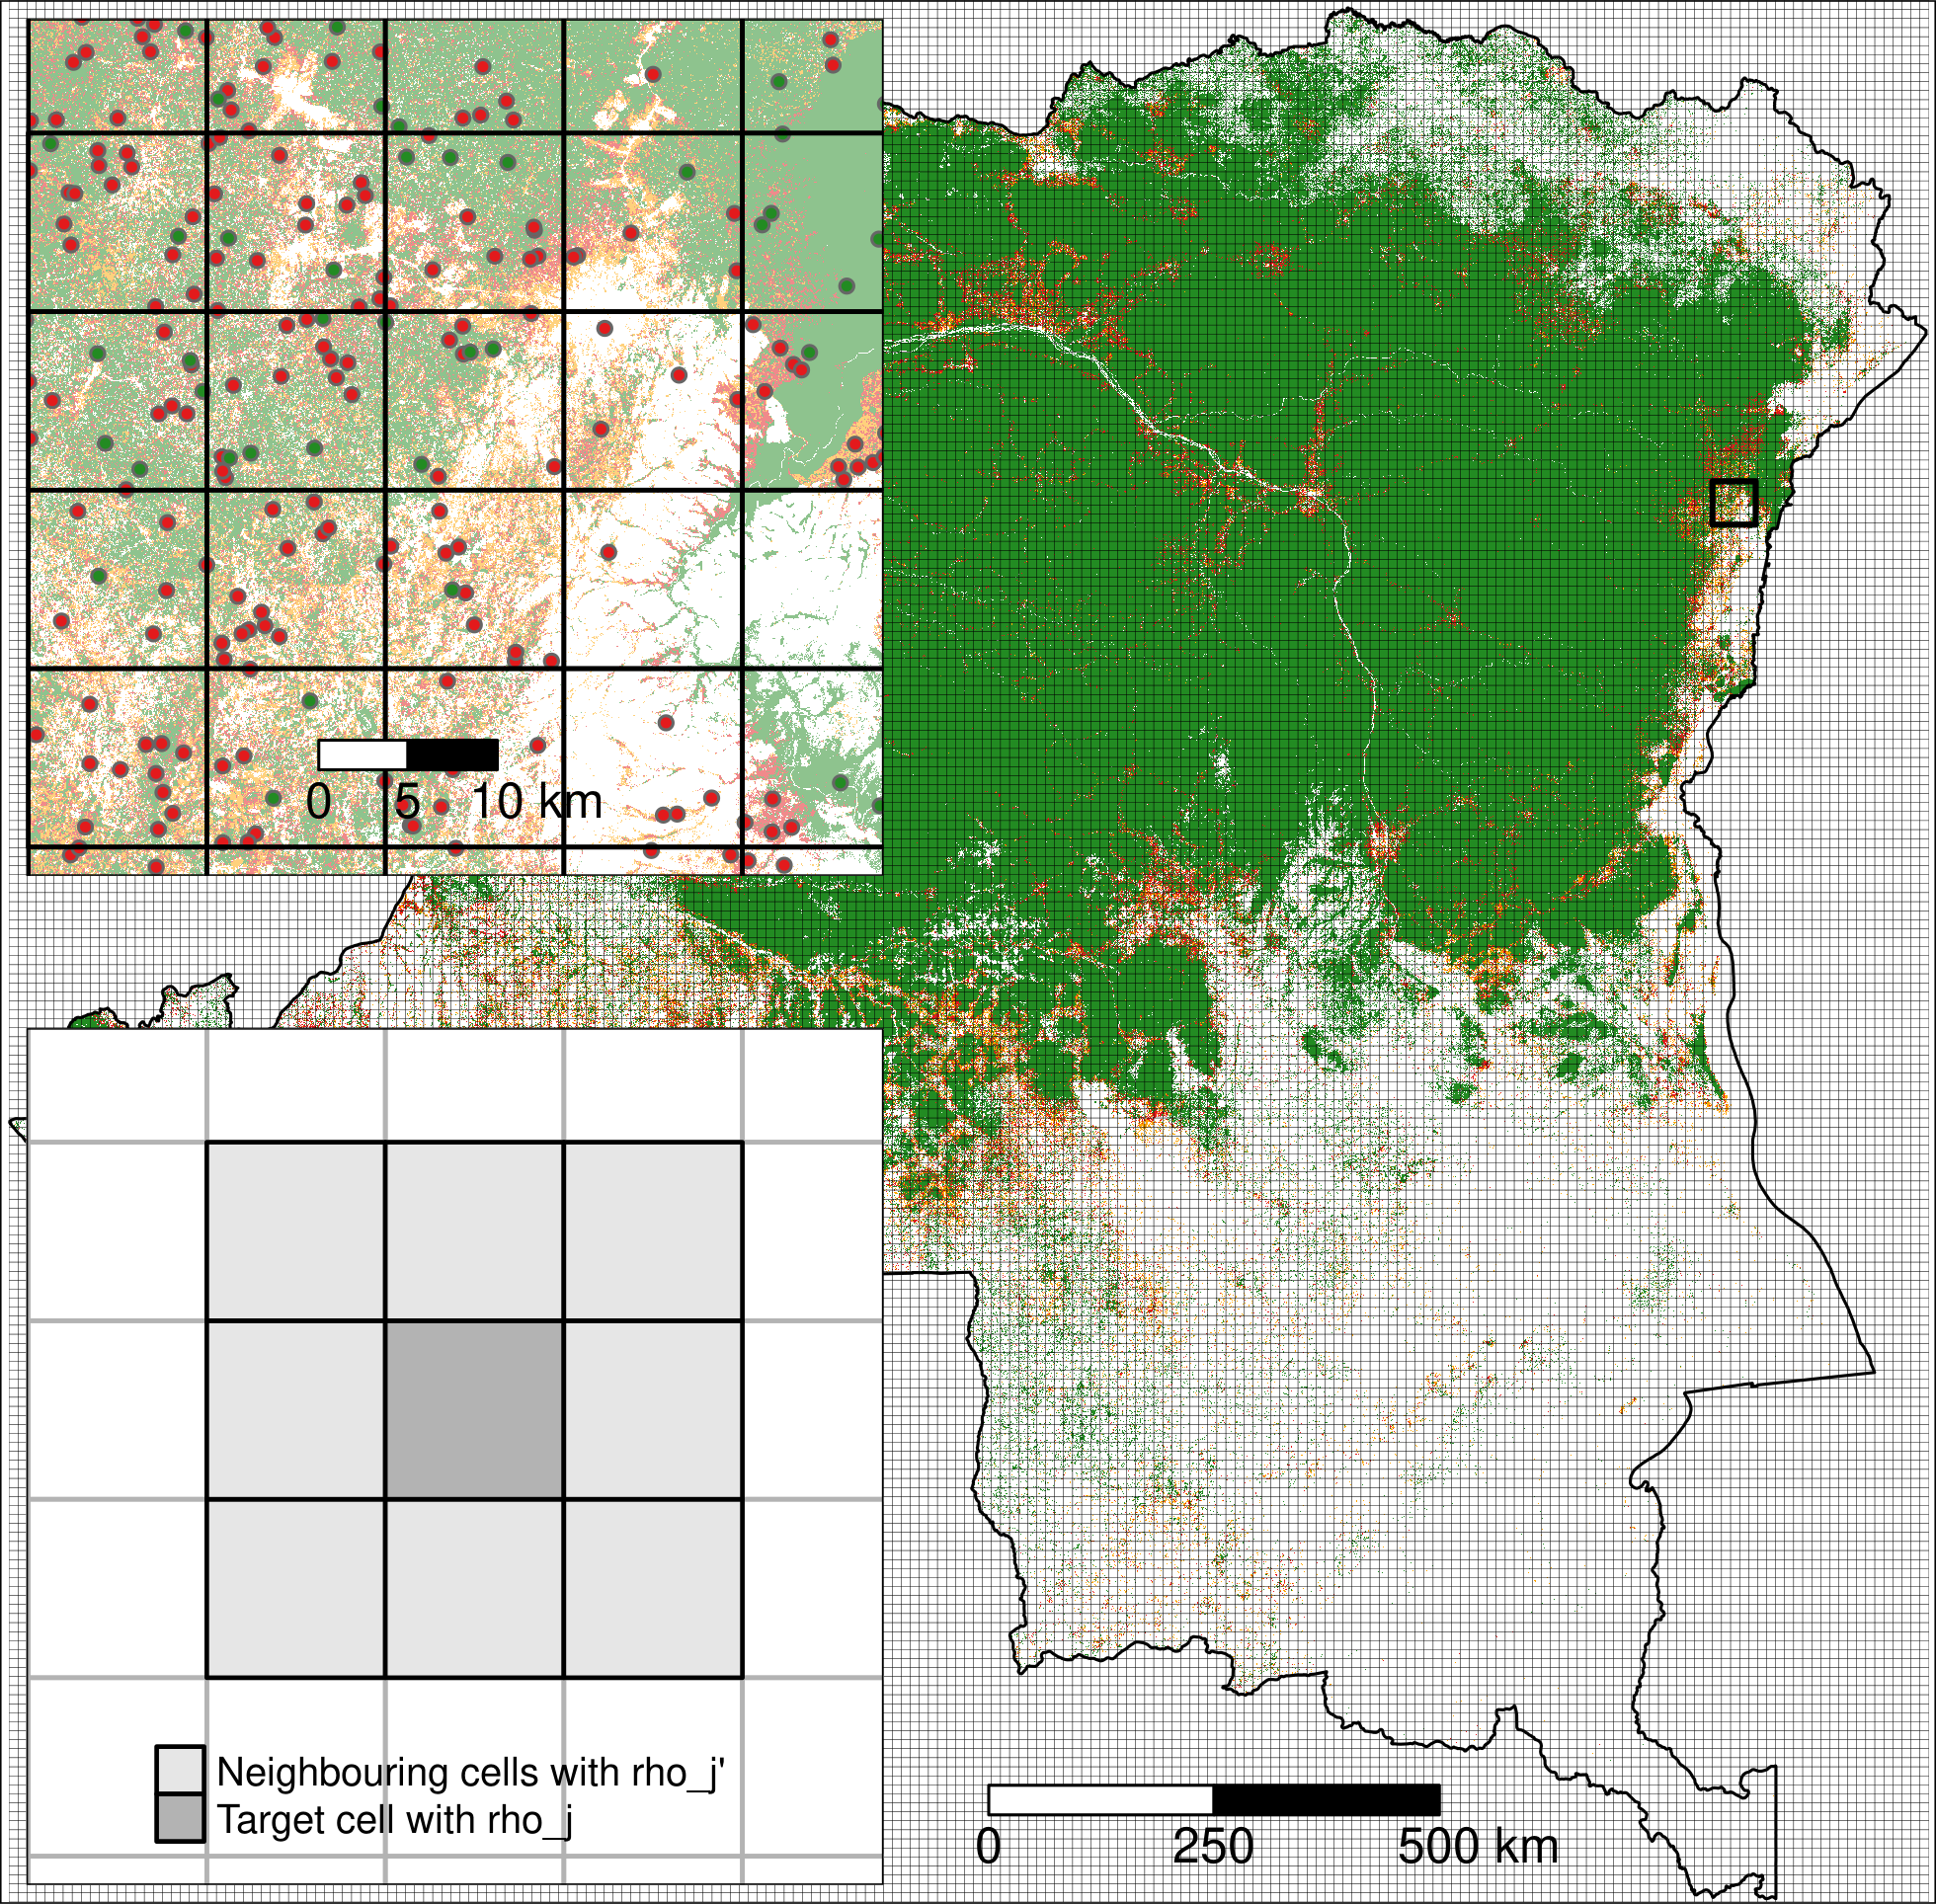
\includegraphics[width=\textwidth]{figs/sm/grid.png}
\end{center}

\textbf{Square grid of 10km cells over DRC}
\end{column}
\end{columns}
\end{frame}

\begin{frame}[label={sec:orgbafa8c3}]{Spatial random effects}
\begin{center}
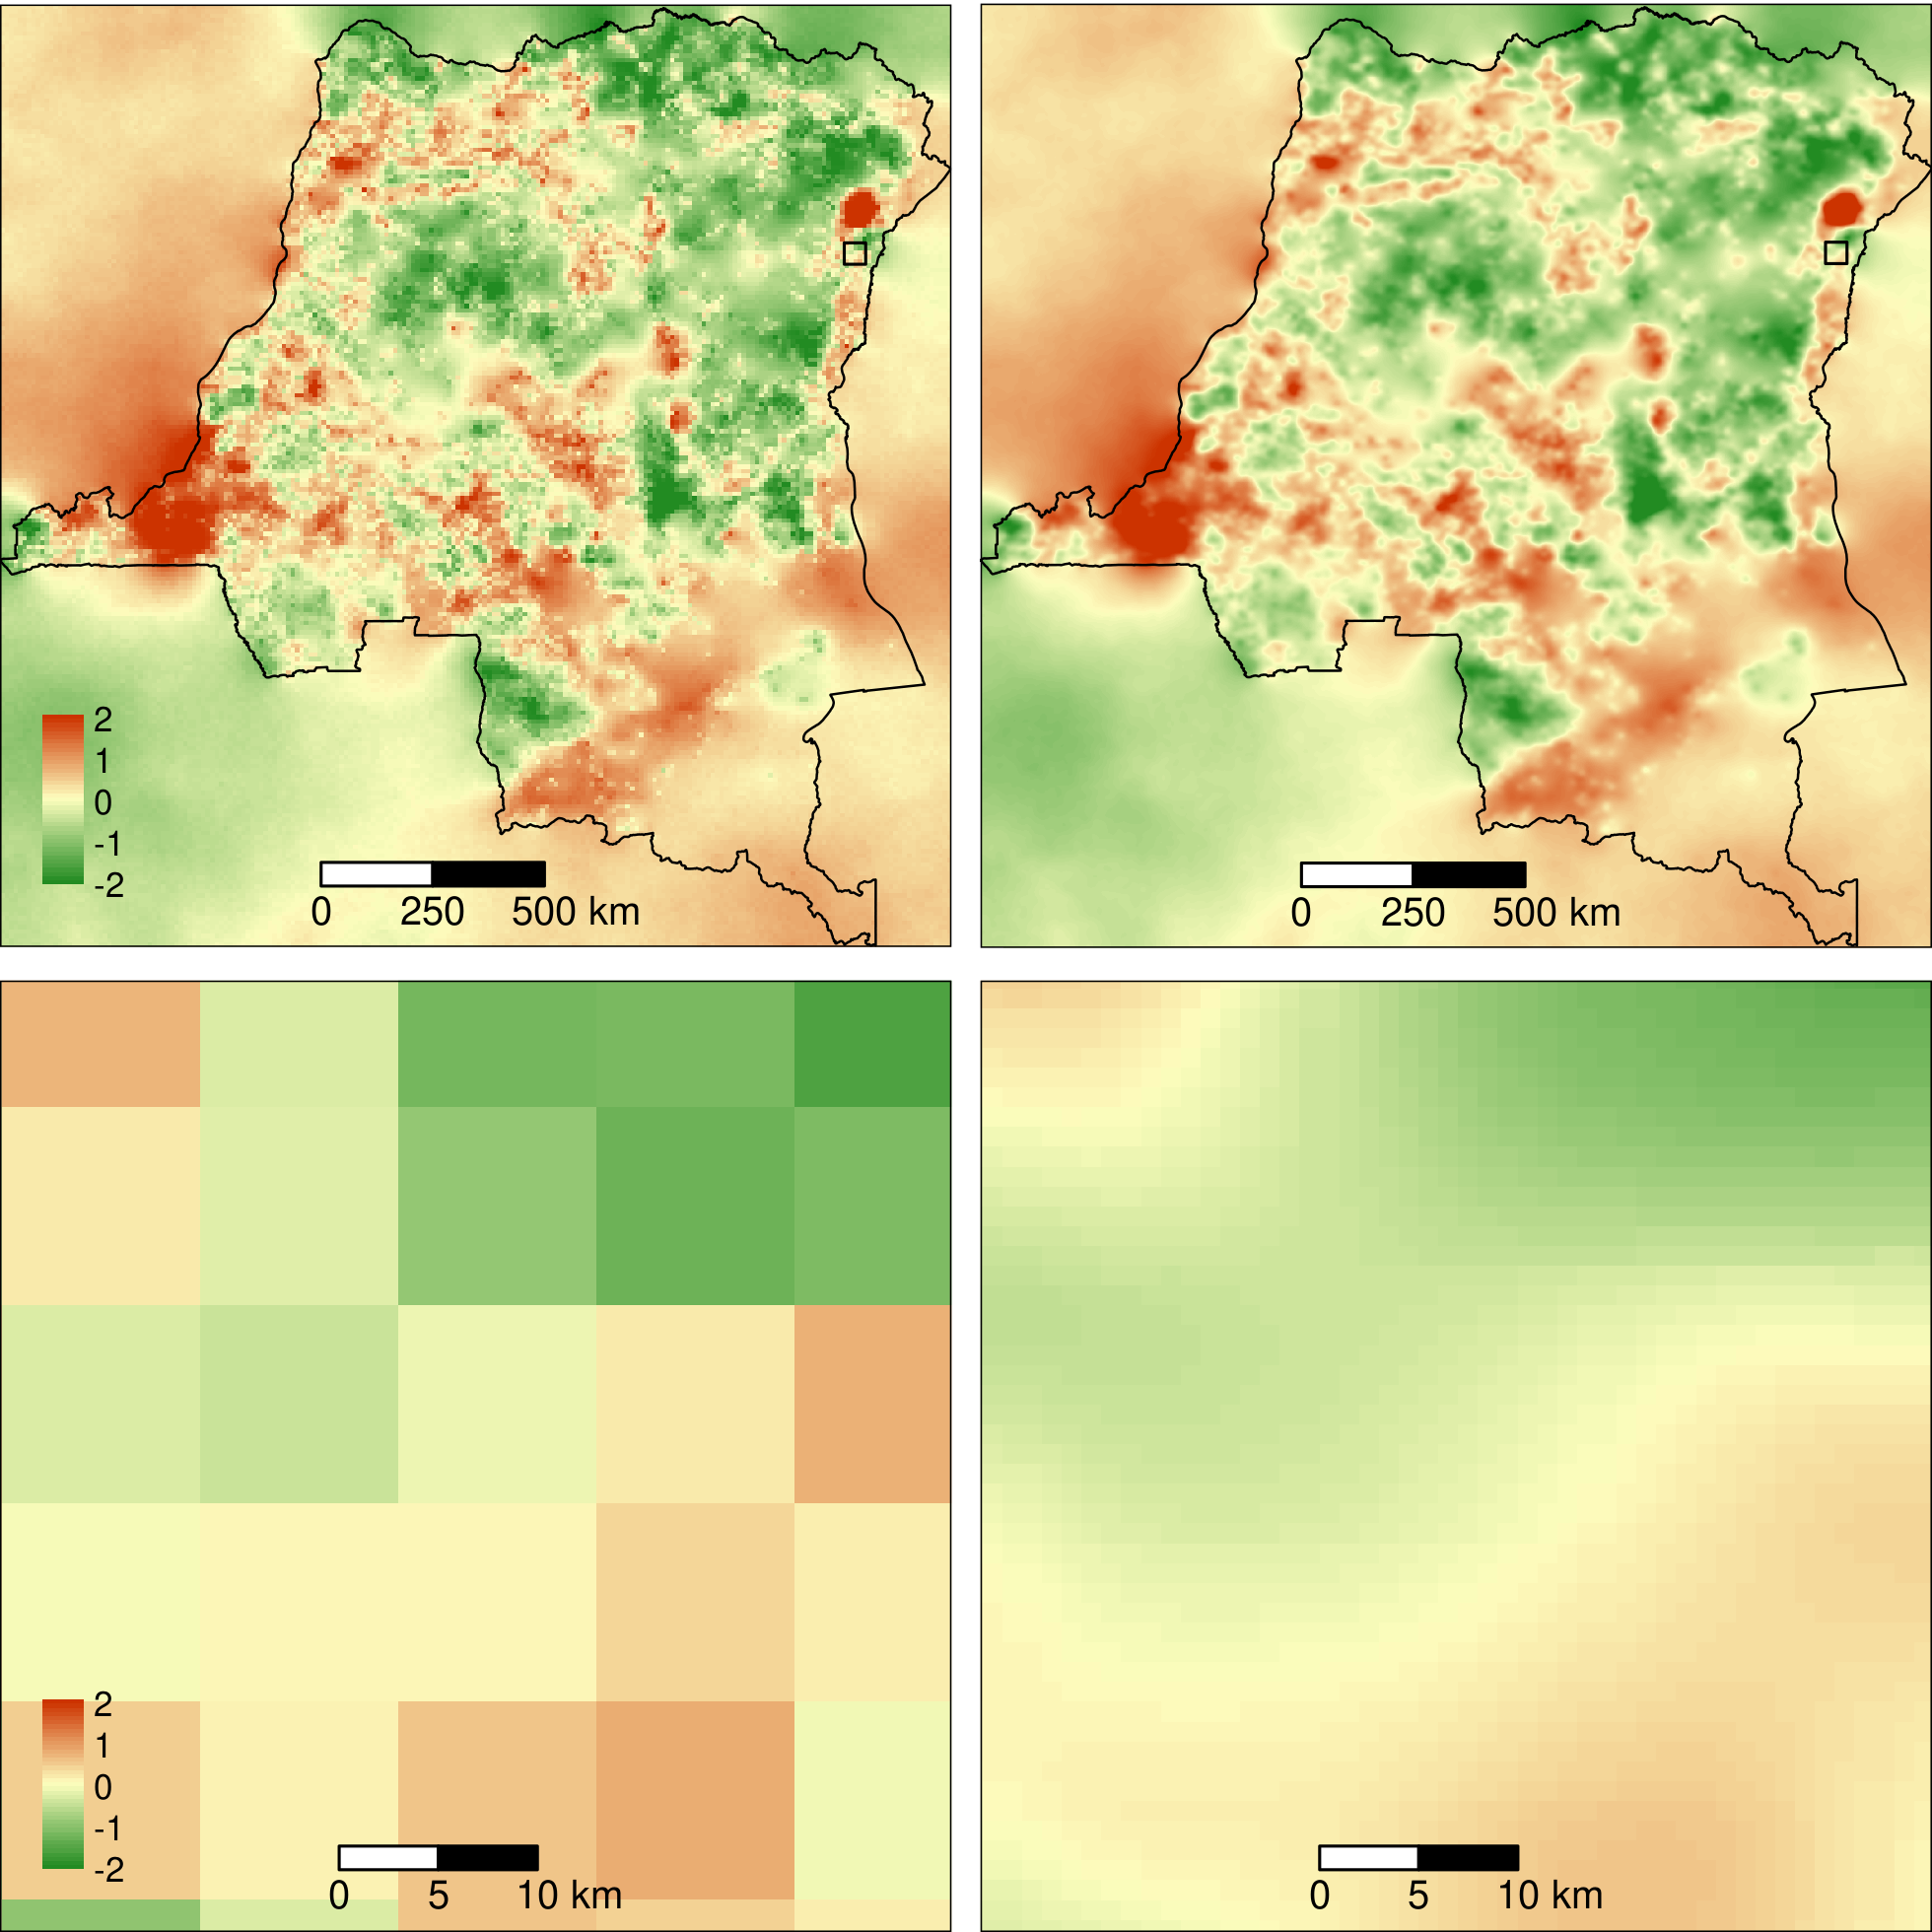
\includegraphics[width=0.6\textwidth]{figs/sm/rho.png}
\end{center}

\textbf{Interpolation of spatial random effects at 1km in DRC}
\end{frame}

\begin{frame}[label={sec:org6d7004f}]{Spatial probability of deforestation}
We use the fitted model to compute the spatial probability of
deforestation.

\begin{center}
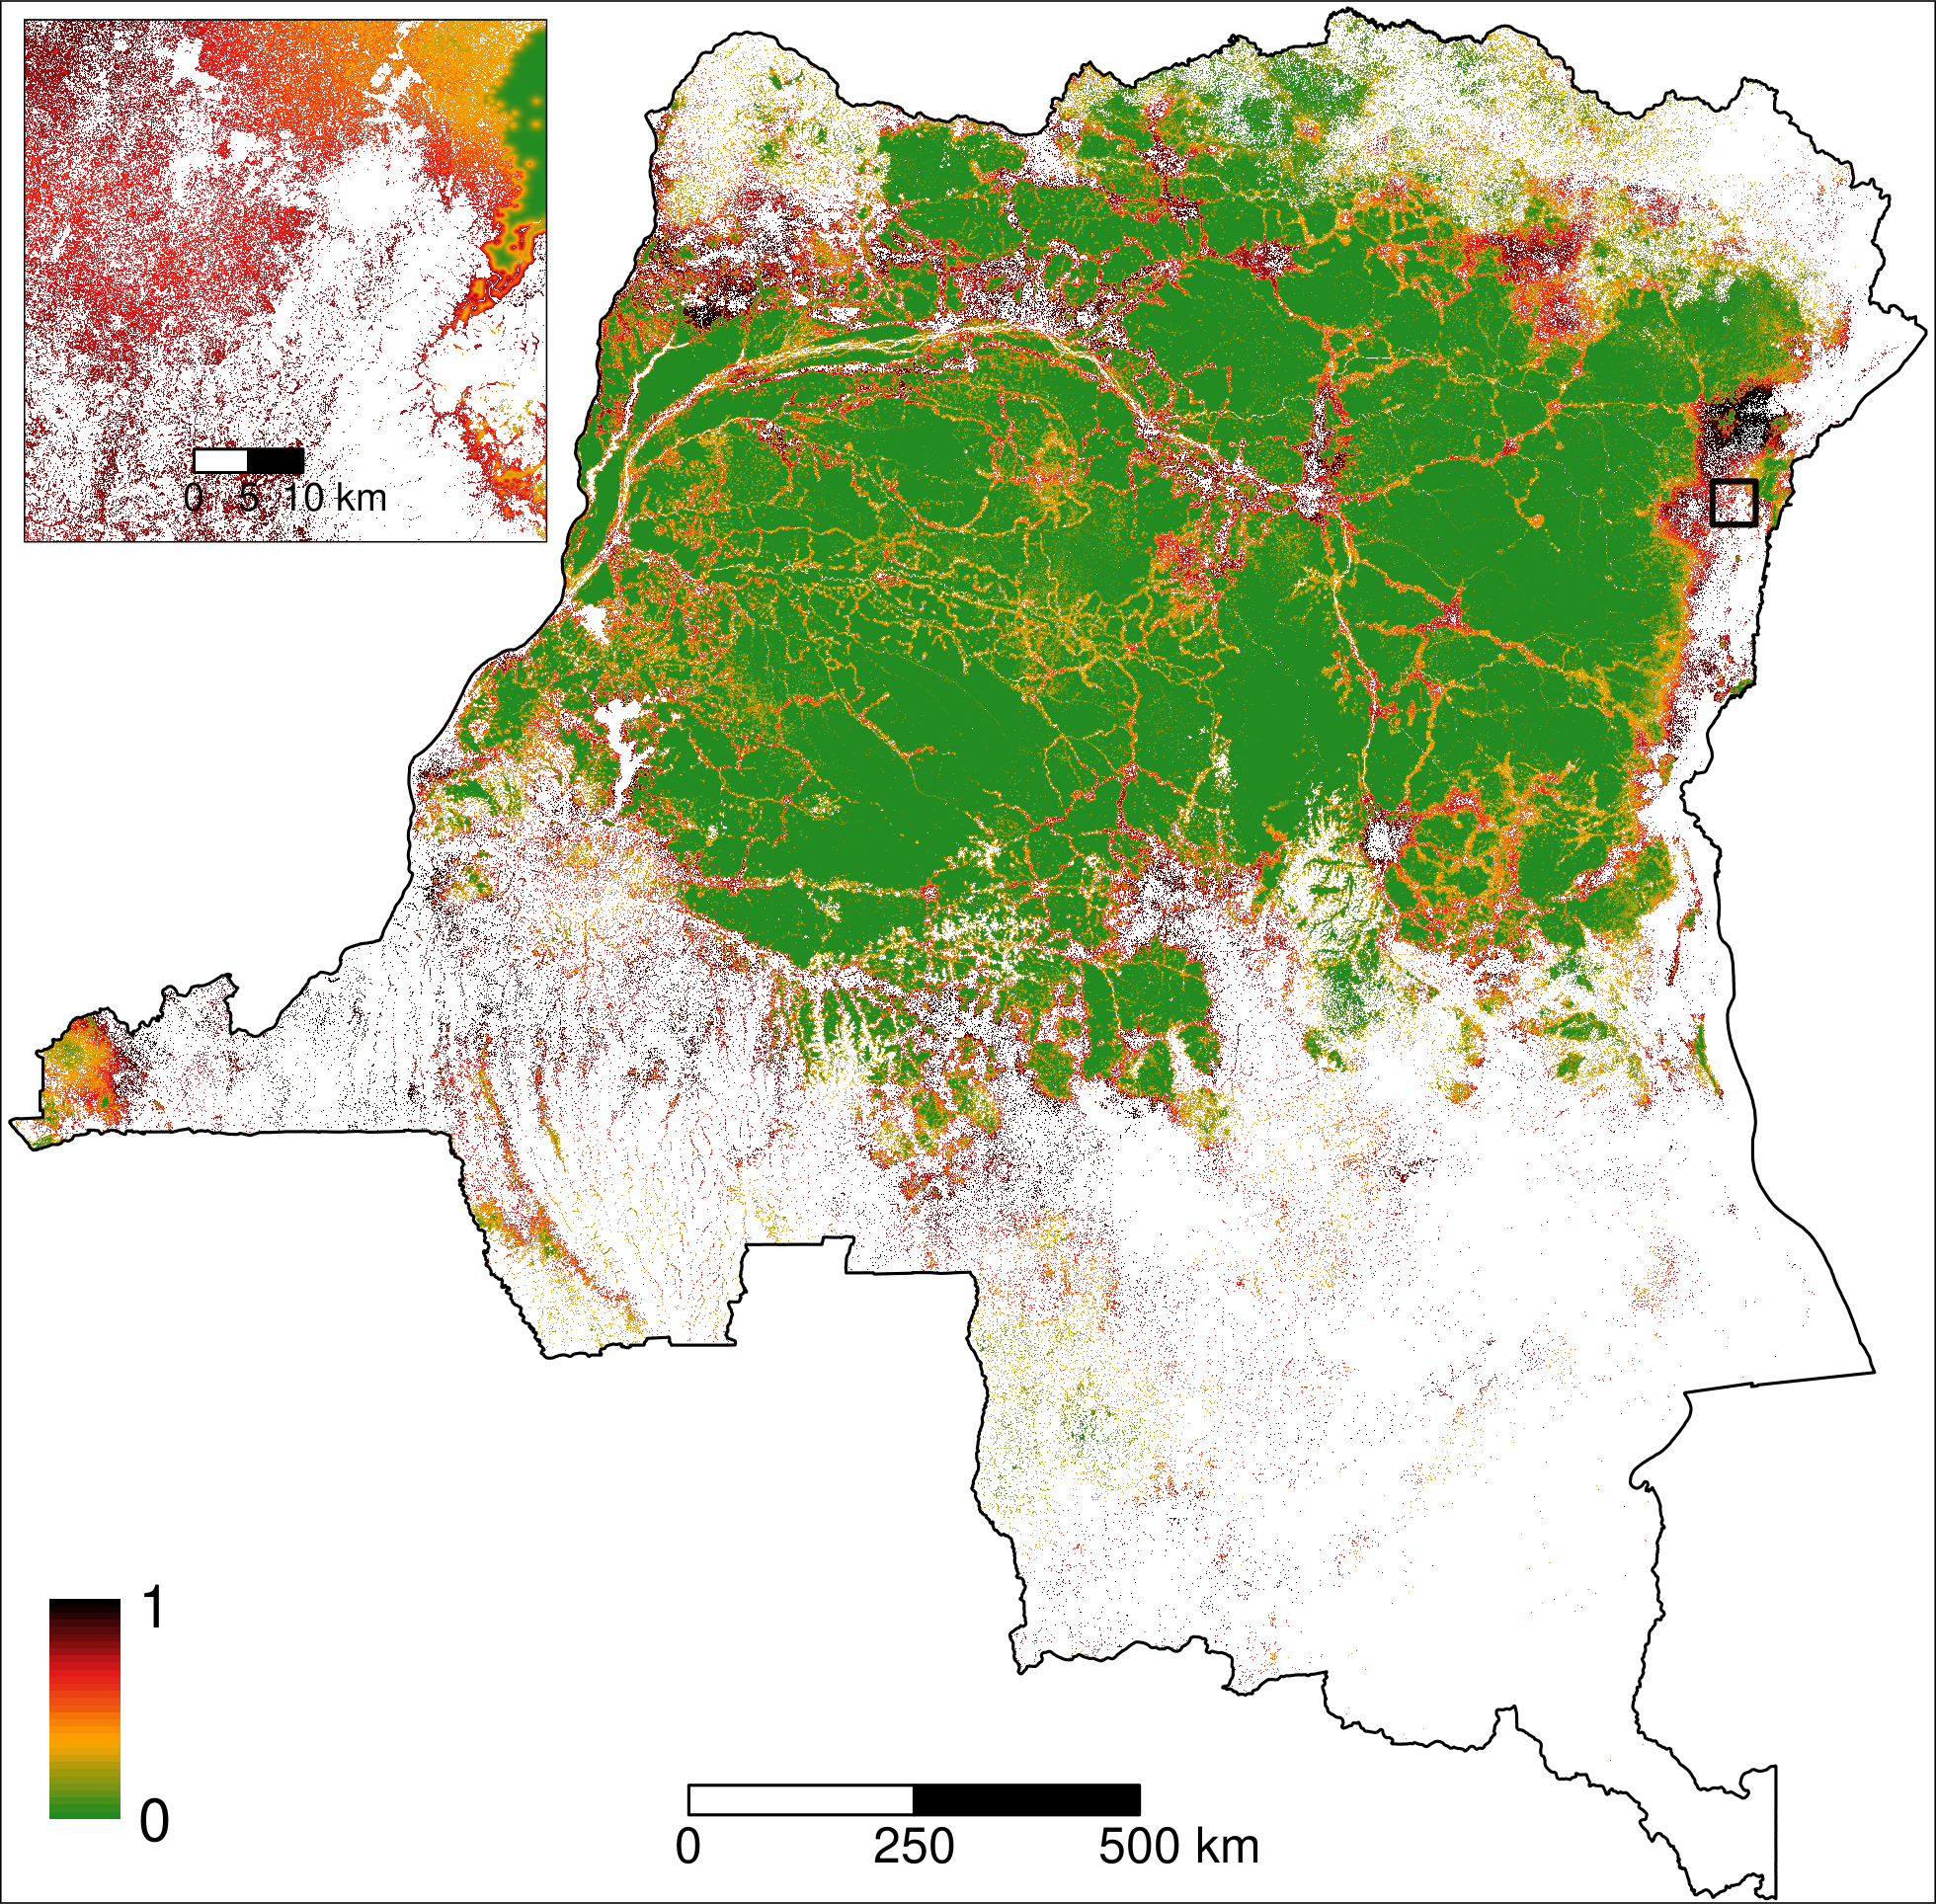
\includegraphics[width=0.5\textwidth]{figs/sm/prob.png}
\end{center}

\textbf{Relative spatial probability of deforestation in DRC for the year 2020}
\end{frame}

\begin{frame}[label={sec:org31c88ab}]{GLM model}
\end{frame}

\begin{frame}[label={sec:orgff7a149}]{Random Forest model}
\end{frame}

\begin{frame}[label={sec:org38f39a7}]{ForestAtRisk in the tropics}
\begin{itemize}
\item \textbf{i.} Consider tropical moist forest in \textbf{92} countries (119 study areas)
\item \textbf{ii.} Estimate the current deforestation rate and uncertainty in each country
\item \textbf{iii.} Model the spatial risk of deforestation from environmental factors
\item \textbf{iv.} Forecast the deforestation assuming a business-as-usual scenario
\item \textbf{v.} Consequences in terms of carbon emissions
\end{itemize}

\vspace{0.5cm}
\begin{center}
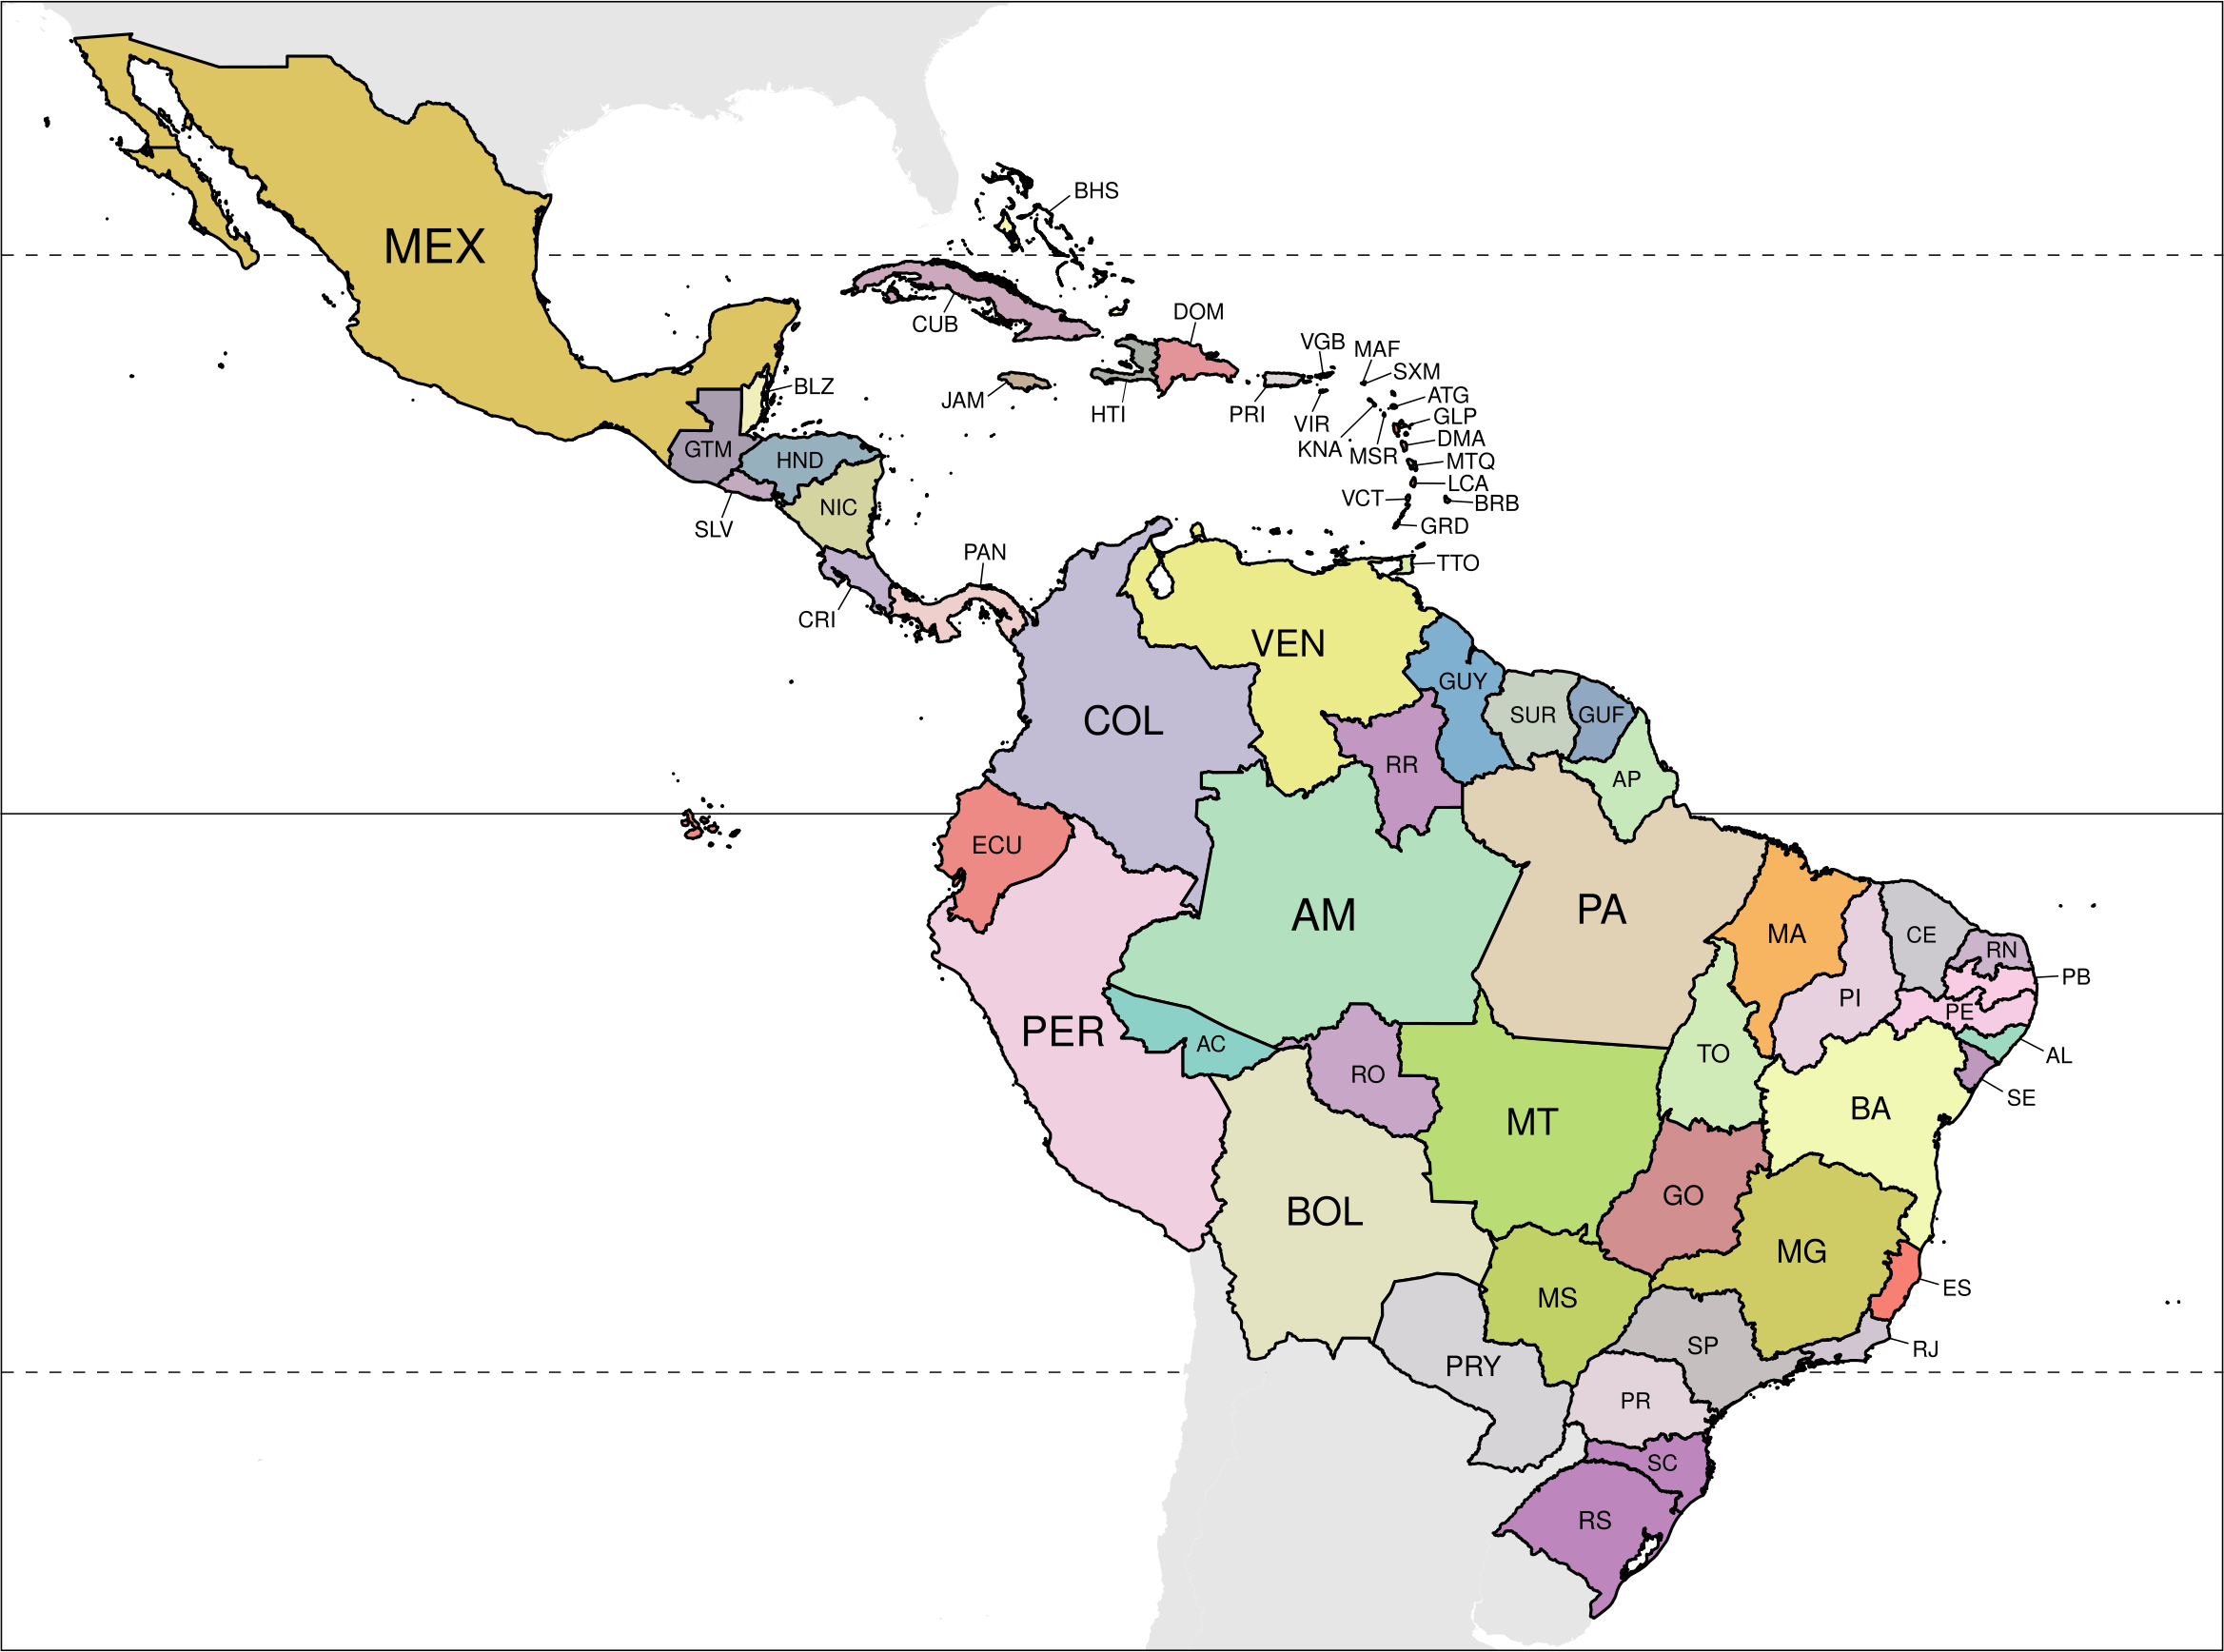
\includegraphics[width=0.32\textwidth]{figs/sm/study_areas_America}
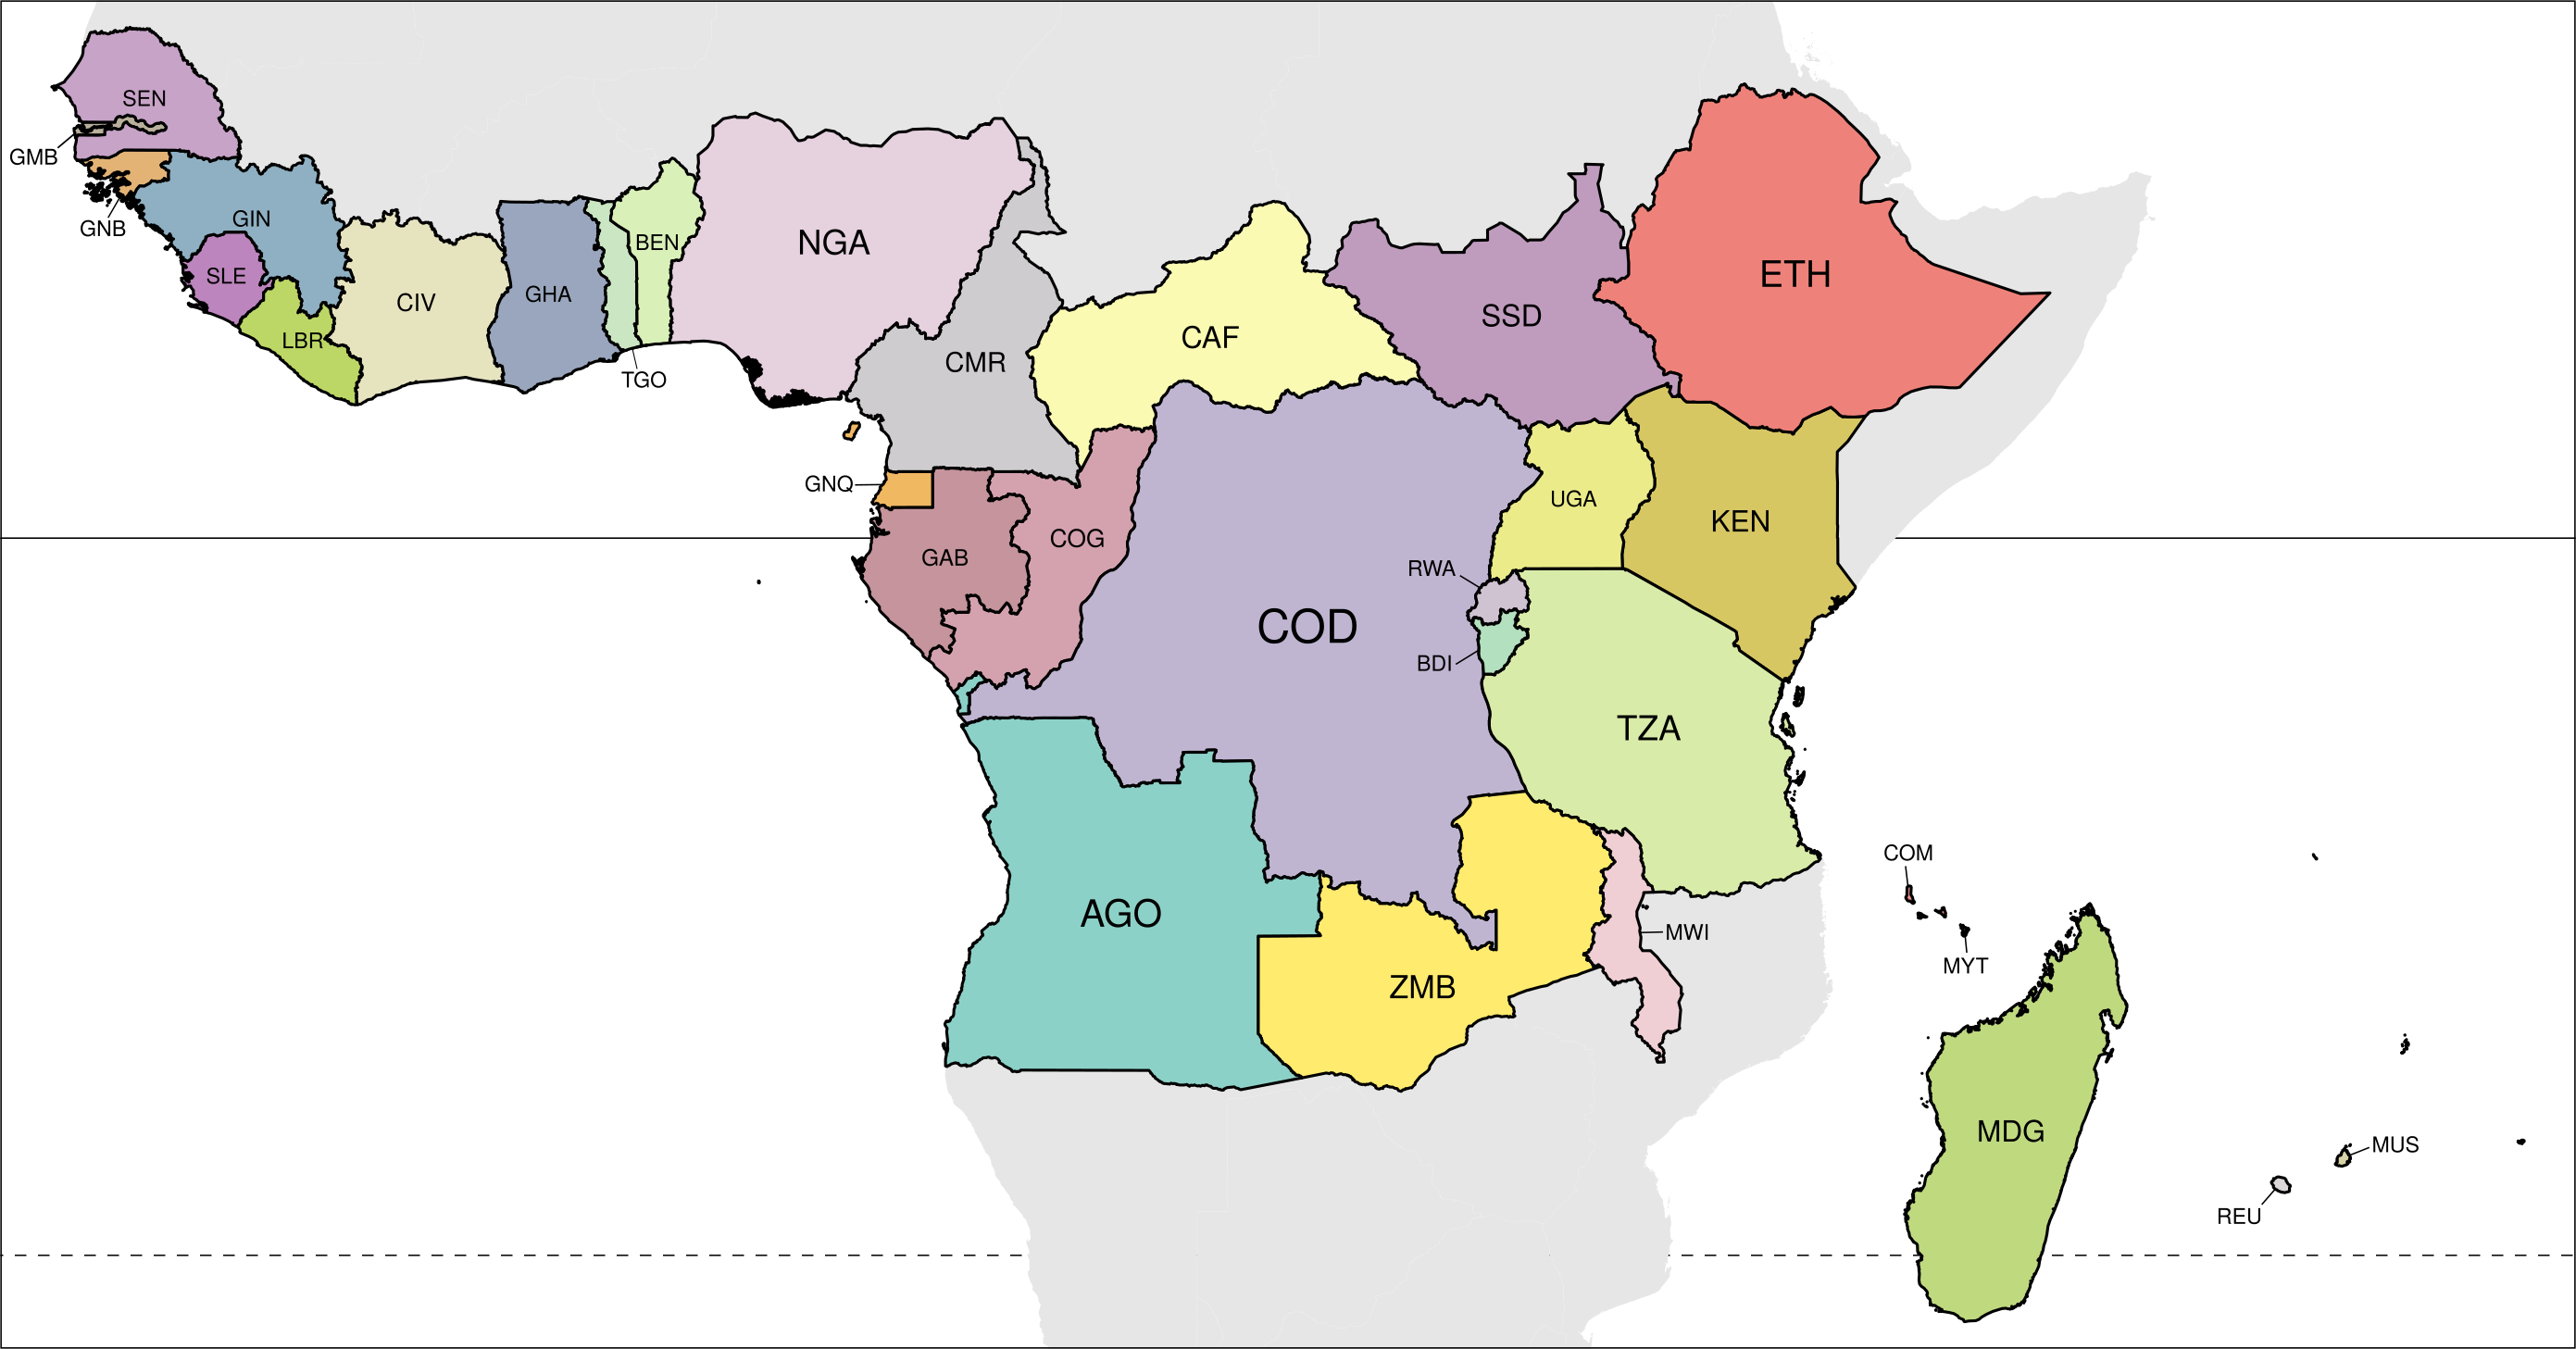
\includegraphics[width=0.32\textwidth]{figs/sm/study_areas_Africa}
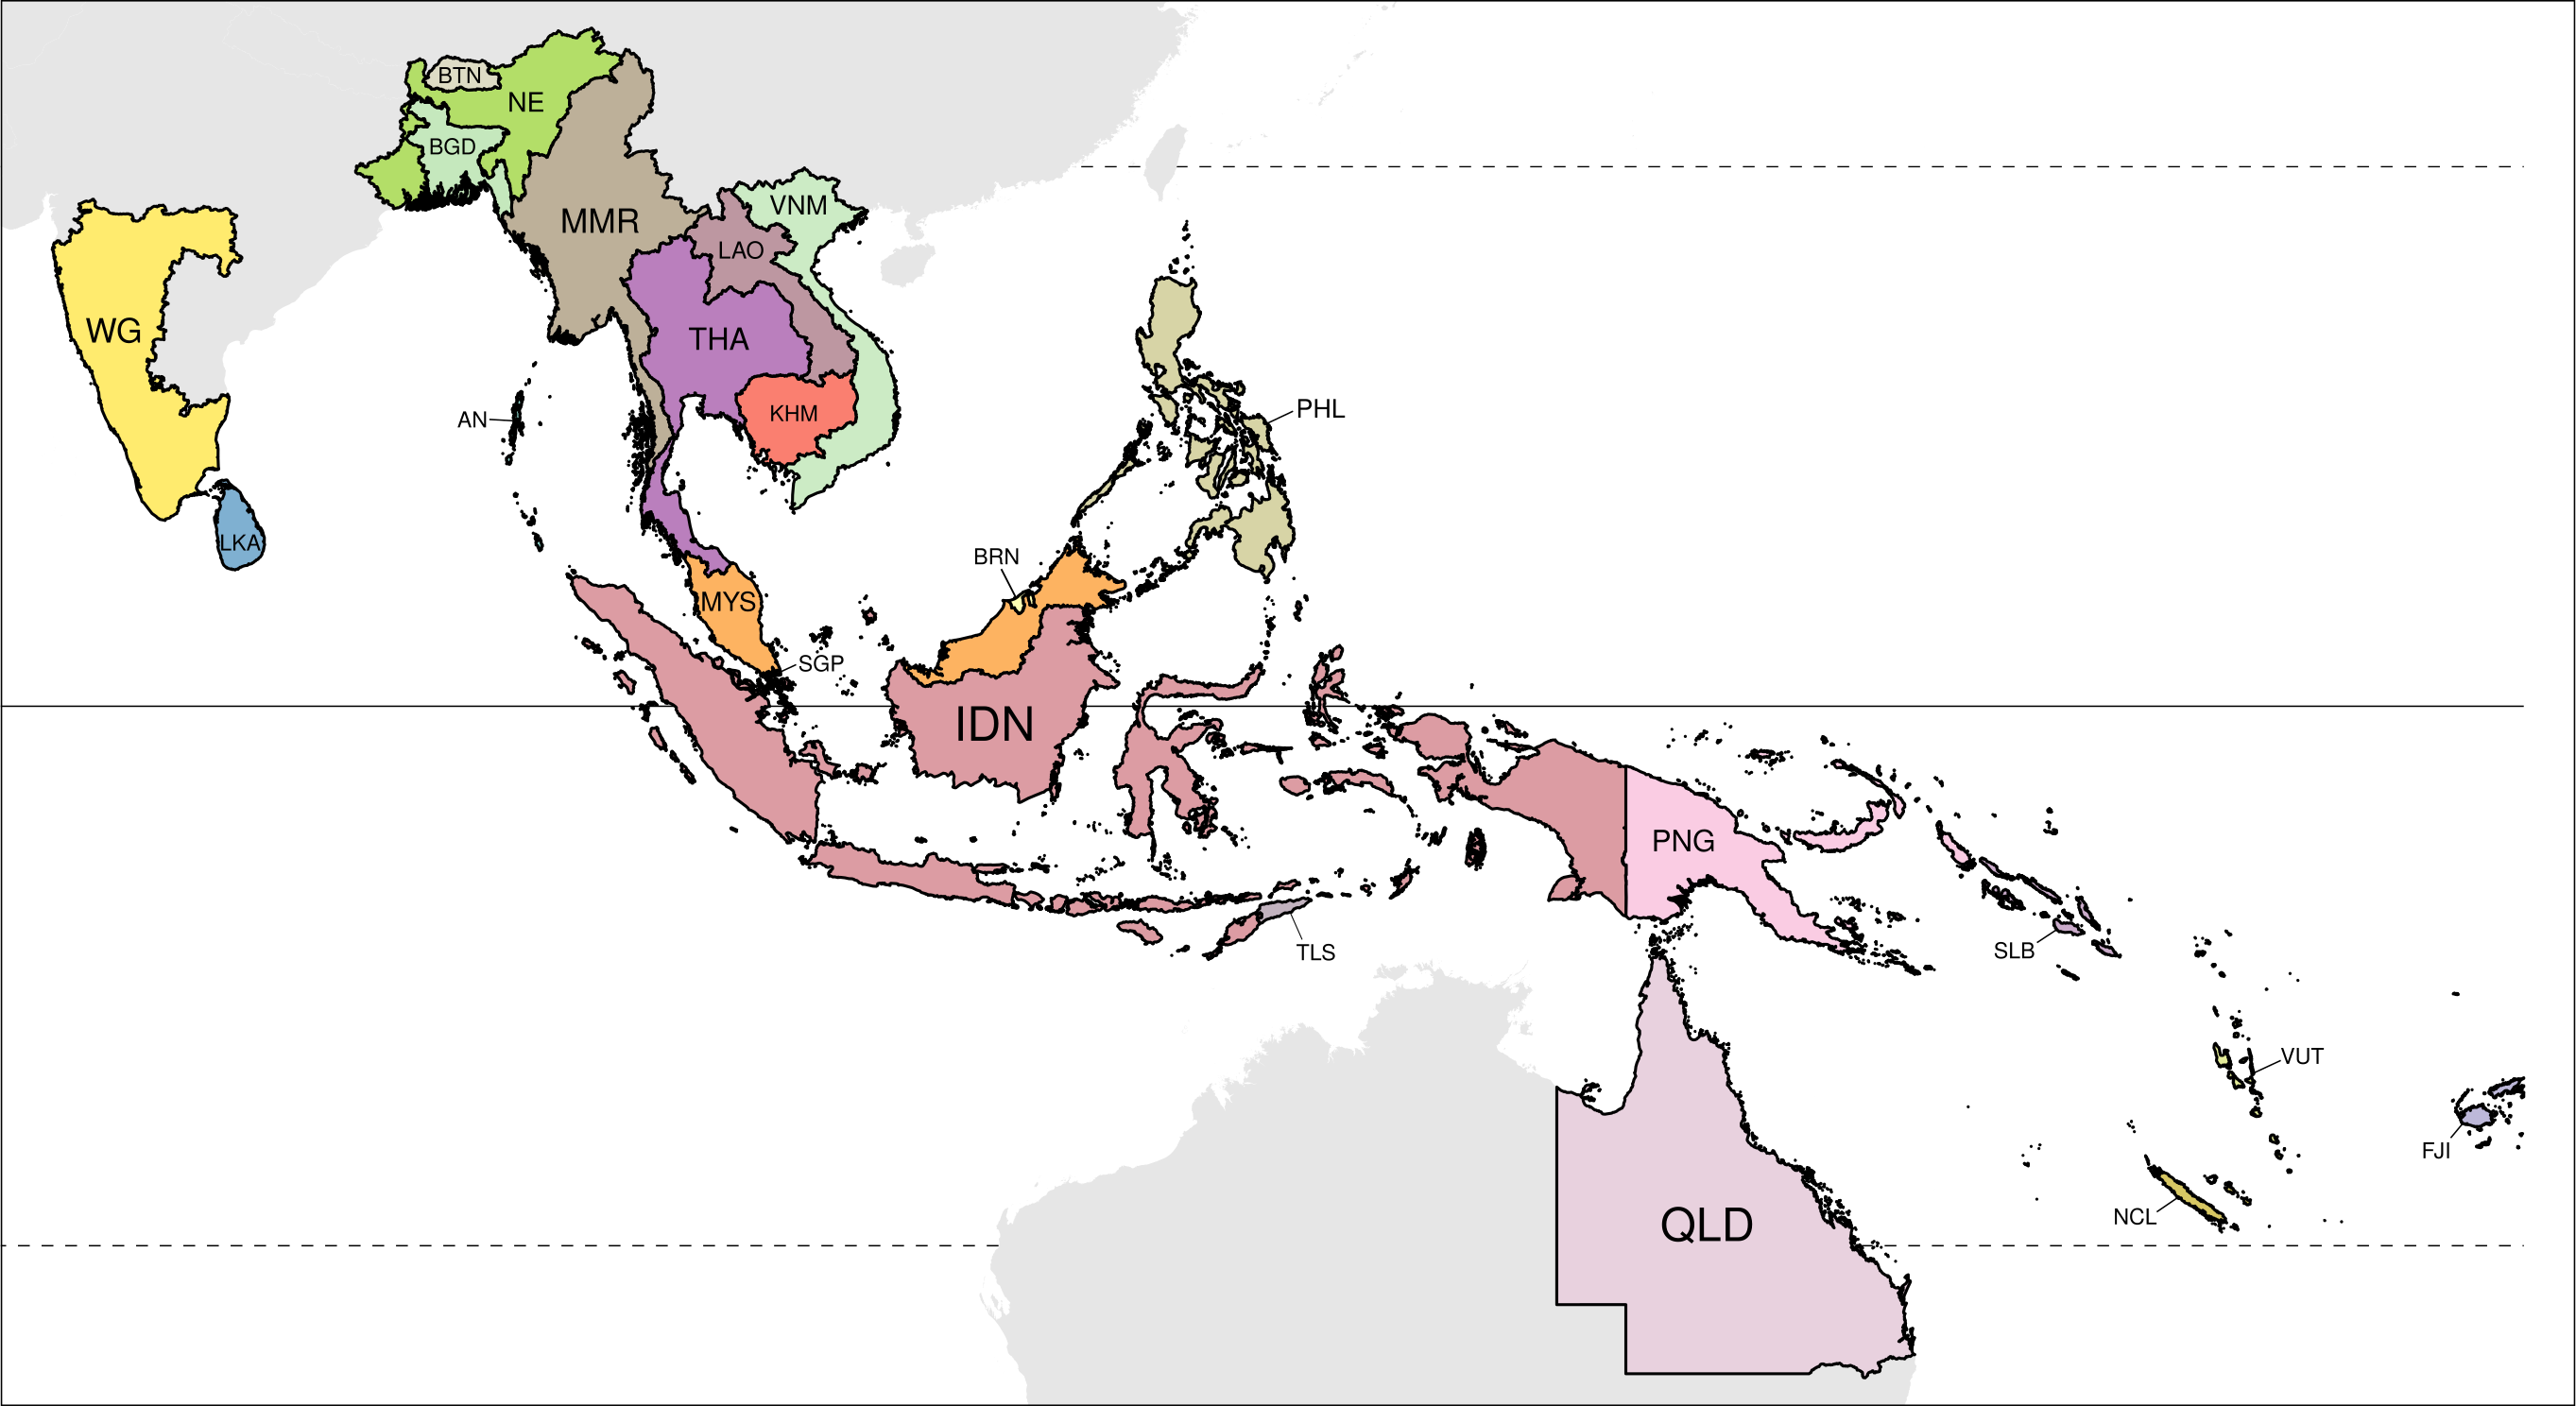
\includegraphics[width=0.32\textwidth]{figs/sm/study_areas_Asia}
\textbf{The 119 study areas in the 3 continents}
\end{center}
\end{frame}

\begin{frame}[label={sec:org6d0c9bb}]{ForestAtRisk in the tropics}
\begin{center}
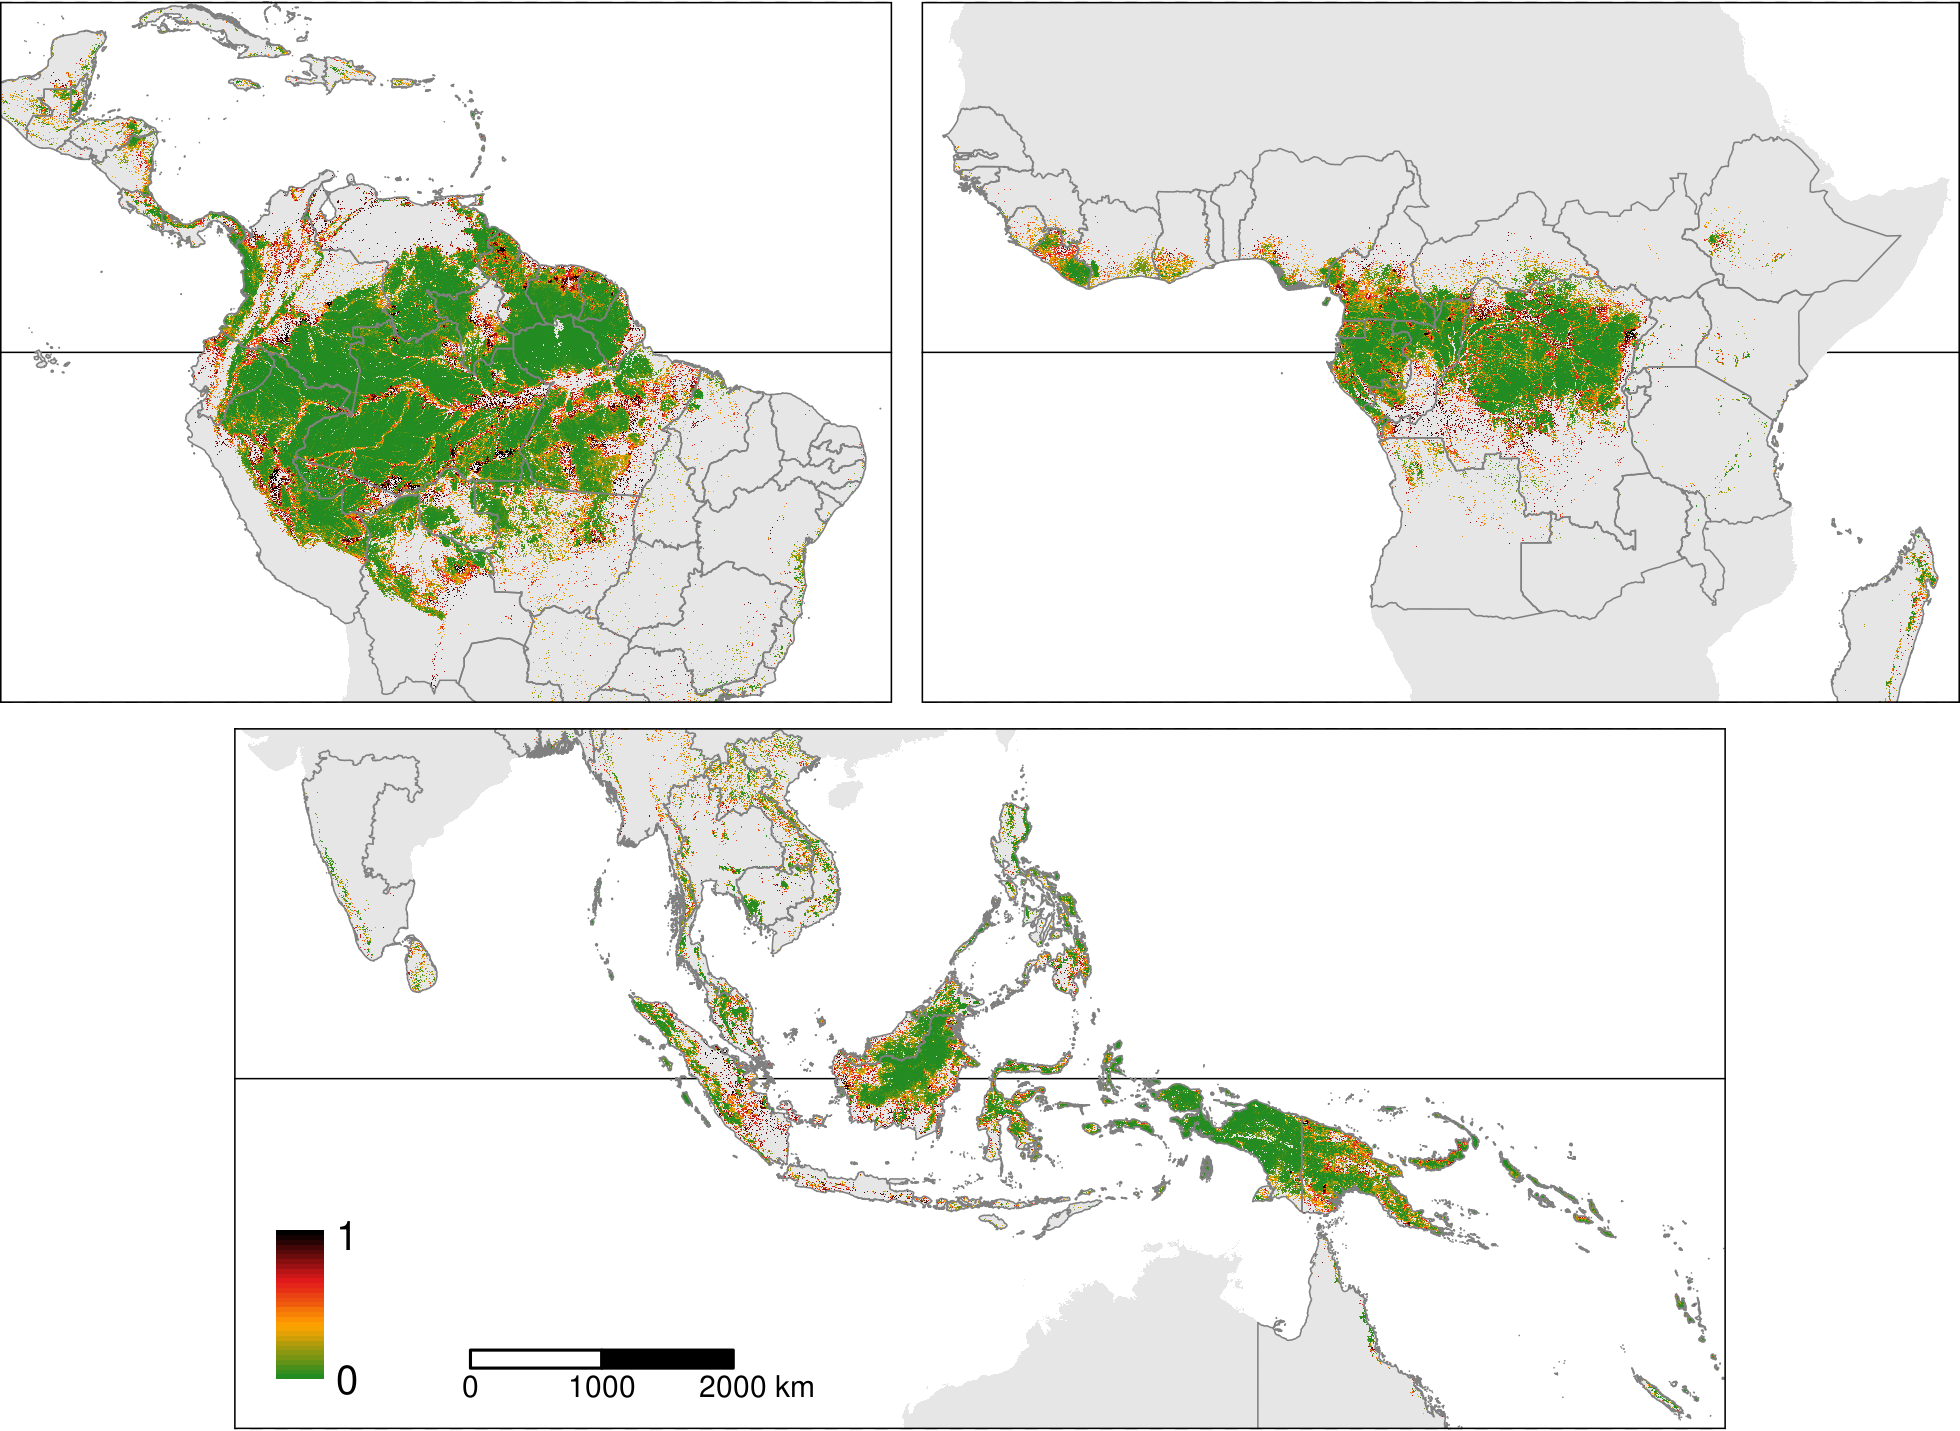
\includegraphics[width=0.7\textwidth]{figs/article/prob.png}
\end{center}

\textbf{Pantropical map of the spatial probability of deforestation}

Article in review: \href{https://doi.org/10.1101/2022.03.22.485306}{10.1101/2022.03.22.485306}

\url{https://forestatrisk.cirad.fr/maps.html}
\end{frame}

\subsection{Moving window models}
\label{sec:org49fd4f6}

\begin{frame}[label={sec:orge573e0a}]{Moving window models}
\end{frame}

\section{Usage}
\label{sec:org3ba92f7}

\subsection{Allocating deforestation}
\label{sec:org5e0ee9a}

\begin{frame}[label={sec:orged23e10}]{Allocating deforestation}
\end{frame}

\subsection{Subnational jurisdictions}
\label{sec:org5d6c8ab}

\begin{frame}[label={sec:org29bc259}]{Subnational jurisdictions}
\end{frame}

\subsection{User's data}
\label{sec:org1d9f05d}

\begin{frame}[label={sec:org126a04c}]{User's data}
\end{frame}

\section{Conclusion}
\label{sec:org4aef317}

\subsection{Week agenda}
\label{sec:orgec453e1}

\begin{frame}[label={sec:org2baf735}]{Week agenda}
\end{frame}

\subsection{Perspectives}
\label{sec:org69dbd4f}

\begin{frame}[label={sec:org122d457}]{Perspectives}
\begin{itemize}
\item Increase computational speed (for predictions on large areas).
\item Adding more alternative models (MLP).
\end{itemize}
\end{frame}

% %%%%%%%%%%%%%%%%%%%%%%%%%%%%%%%%%%%%%%%%%%%%%%%%%%%%%%%%%%

{
  % Use background image
  \usebackgroundtemplate{%
    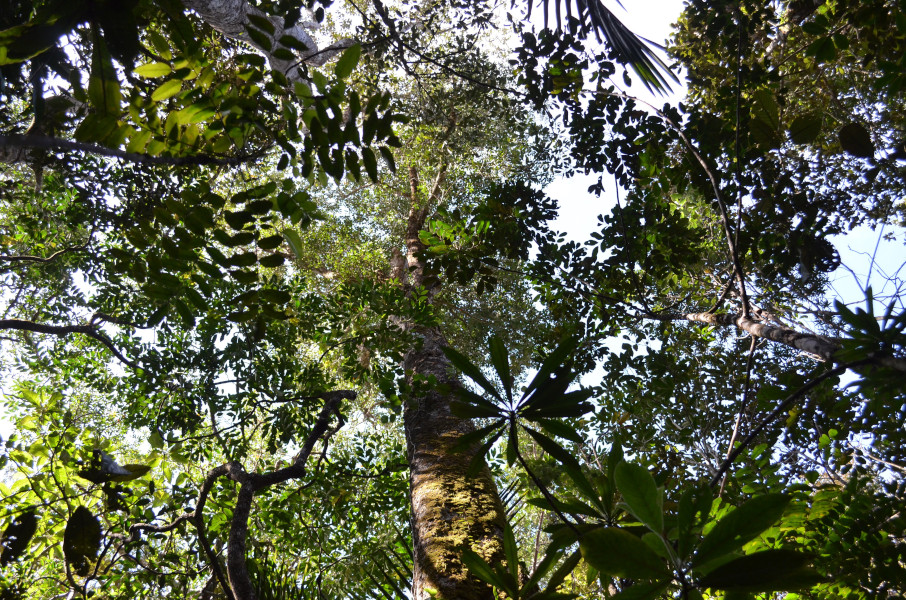
\includegraphics[keepaspectratio=true, height=\paperheight]{figs/Canopy-NC}
  }
  \setbeamertemplate{navigation symbols}{}
  % Remove shadow from block
  \setbeamertemplate{blocks}[rounded][shadow=false]
  \begin{frame}[plain]
  	\vspace*{\stretch{100}} 
    \begin{block}{}
      \begin{center}
        \ldots~Thank you for attention~\ldots \\
        \url{https://ecology.ghislainv.fr/deforisk-qgis-plugin} \\
        \textbf{> Articles > References > Presentations} \\
        
\includegraphics[width=0.8\textwidth]{figs/partners_logos}
      \end{center}
    \end{block}
  \end{frame}
}
\end{document}
